Inteligencia Artificial \index{Inteligencia Artificial} se refiere a la
habilidad de las máquinas de hacer cosas que se presupone requieren
inteligencia. Es un intento de descubrir y describir los aspectos humanos del
intelecto y abstraer aquellos que puedan ser simulados por las máquinas. También
podemos pensar este concepto como un intento de desarrollar una teoría
matemática que describa las capacidades de las cosas (naturales o artificiales)
que exhiben un \emph{comportamiento inteligente}. 

Como área multidisciplinaria, la \hyperlink{abbr}{IA} también tiene dentro de su espectro
cuestiones filosóficas y metafísicas que guían el desarrollo de la
investigación. Estos son algunos ejemplos de preguntas filosóficas que se
plantean dentro de la \hyperlink{abbr}{IA}:

\begin{itemize}
    \item ¿Que se conoce como Inteligencia Natural?
    \item ¿Cuándo podemos describir como inteligente a una máquina?
    \item ¿Cuál es el grado en el cual las máquinas exhiben o simulan comportamiento inteligente?
    \item ¿Las máquinas podrán, eventualmente, simular inteligencia?
    \item ¿Cómo las máquinas y su comportamiento puede ser modelado matemáticamente?
    \item ¿Qué usos podría tener una máquina inteligente?
\end{itemize}

Tradicionalmente, la \hyperlink{abbr}{IA} se ha enfocado en las siguientes aplicaciones:
Percepción de Patrones, Probar Teoremas, Procesamiento de Lenguaje Natural e
Información Semántica, Cómputo Evolutivo e Inspirado por la Naturaleza,
Razonamiento y Resolución de Problemas. \cite{Jackson1985}

En la \autoref{fig:tecnicas-ia} se cuenta con una clasificación sencilla de los
algoritmos que componen la \hyperlink{abbr}{IA}. Estas clasificaciones pueden
combinarse para generar nuevos algoritmos que se comporten o contengan
componentes distintos.

\begin{figure}[H]
    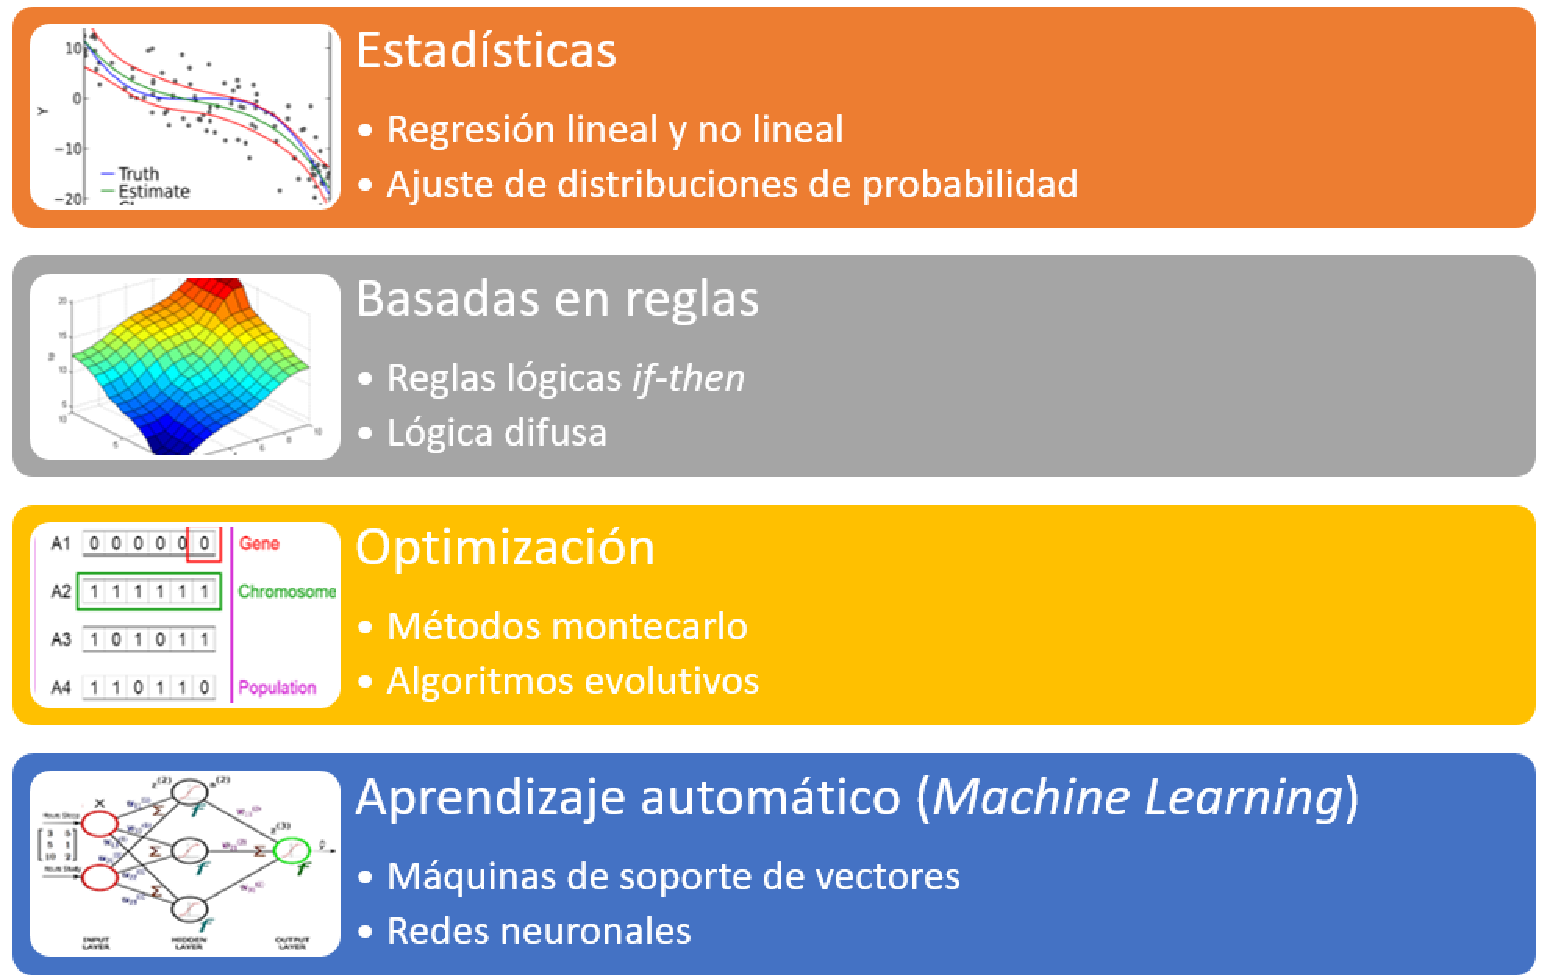
\includegraphics[width=\textwidth,height=0.9\textheight,keepaspectratio]{capitulo_marcoteorico/tecnicas}
    \caption{Técnicas y ejemplos de Inteligencia Artificial}\label{fig:tecnicas-ia}
\end{figure}

\begin{enumerate}
    \item{\textbf{Estadísticas: }} Se toman como técnicas estadísticas aquellas que han sido basadas en una perspectiva
    matemática rigurosa e incluyen algoritmos clásicos basados en Mínimos Cuadrados hasta algoritmos modernos
    como los modelos de mezcla Gaussiana.
    \item{\textbf{Basadas en reglas: }} Son las que potenciaban los esfuerzos en la investigación de Sistemas Expertos
    y tienen algoritmos que son capaces de manejar la incertidumbre así como variables lingüísticas.
    \item{\textbf{Optimización: }} Estas toman una función y buscan los parámetros para buscar el resultado óptimo deseado.
    Incluyen a las llamadas \emph{metaheurísticas} así como modelos probabilísticos capaces de manejar riesgo.
    \item{\textbf{Aprendizaje Automático: }} Conocido como ML, es el conjunto de algoritmos más prometedores dentro de la AI
    ya que son capaces de extraer información contenida en los datos y proveer de modelos sumamente robustos de predicción.
\end{enumerate}

\subsection{Procesamiento Digital de imágenes}

Procesar una imagen, implica aplicar ciertas operaciones en ella para cambiar
sus propiedades tales como nitidez, contraste así como para extraer información
de ella o mejorar su calidad. Estrictamente, el procesamiento de imágenes es una
forma de procesar una señal \(x\), la cual entra a un proceso \(p(x)\) y nos
devuelve ya sea una imagen \(x'\) o el conjunto de características que la
componen \(\mathbf{x}\).~\cite{UniversityofTartu}

A \emph{grosso modo}, el \hyperlink{abbr}{PDI} se reduce a los siguientes
pasos:

\begin{itemize}
    \item Adquirir imagen.
    \item Manipular imagen.
    \item Resultados.
\end{itemize}

Las señales se dividen en digitales y analógicas. Las señales analógicas
son aquellas que siguen un espectro continuo, un ejemplo de imágenes
analógicas son las fotografías o los rayos X. Sin embargo, en el área
de Ciencias de la Computación y la \hyperlink{abbr}{IA}, trabajaremos
con señales digitales, que son aquellas que se pueden representar con matrices de números.

\subsubsection{Enfoque}

El \hyperlink{abbr}{PDI}, como mencionamos anteriormente, consiste en capturar
una imagen en un dispositivo electrónico y aplicarle algoritmos y funciones
matemáticas ya sea para mejorarla para interpretación humana o extraer
información automáticamente. Ofrece muchas ventajas con respecto al
procesamiento de imágenes analógicas ya que reduce el ruido y la distorsión de
la señal. 

El \hyperlink{abbr}{PDI} tiene dos objetivos \cite{Forsyth2012}:

\begin{itemize}
    \item Mejorar la información pictórica de la imagen para su interpretación
    humana.
    \item Procesar la imagen para su almacenado, transmisión o proceso por
    algoritmos autónomos de percepción.
\end{itemize}

\begin{figure}[H]
    \centering
    \begin{tikzpicture}
        \node[block] [rectangle split, rectangle split parts=4, minimum size=4cm, text centered, text width=4cm] (a) { \textbf{Procesamiento de nivel bajo}
        \nodepart{second}
            \textbf{Entrada:} Imagen
        \nodepart{third}
            \textbf{Salida:} Imagen
        \nodepart{fourth}
            \textbf{Ejemplo: } Remoción de ruido, mejora de nitidez
        };
        \node[block,right=of a] [rectangle split, rectangle split parts=4, minimum size=4cm, text centered, text width=4cm] (b) {\textbf{Procesamiento de nivel medio}
        \nodepart{second}
            \textbf{Entrada:} Imagen
        \nodepart{third}
            \textbf{Salida:} Atributos y características
        \nodepart{fourth}
            \textbf{Ejemplo:} Reconocimiento de objetos, segmentación
        };
        \node[block,right=of b] [rectangle split, rectangle split parts=4, minimum size=4cm, text centered, text width=4cm] (c) {\textbf{Procesamiento de nivel alto}
        \nodepart{second}
            \textbf{Entrada:} Atributos y características
        \nodepart{third}
            \textbf{Salida:} Entendimiento
        \nodepart{fourth}
            \textbf{Ejemplo:} Navegación autónoma, reconocimiento facial
        }; 
        \draw[line] (a)--(b);
        \draw[line] (b) --(c);
      \end{tikzpicture}
      \caption{Las imágenes y su procesamiento}
      \label{fig:dpi}
\end{figure}

Hasta hace algunas décadas, esta parte del \emph{entendimiento} de una imagen
era realizada por algoritmos bastante complejos y específicos, generalmente con
un único propósito. La tesis propone reemplazar estos algoritmos por DL no solo
para facilitar la creación de sistemas de VC sino porque ConvNets también tienen
mejor precisión y se desempeñan mejor en el mundo real. 

Es por ello que usaremos el \hyperlink{abbr}{PDI} como un método para capturar y preparar imágenes
o video para posteriormente alimentar a la ConvNet ya entrenada y para la
manipulación y preprocesamiento de las imágenes para entrenar la red. 

\subsubsection{Orígenes}

Los periódicos, en la década de 1920 (\autoref{fig:dpiearly}), fueron de los
pioneros en la aplicación de imágenes digitales. Podían transmitir imágenes a
través del Océano Atlántico mediante cable submarino, mientras que equipo
especializado decodificaba la imagen y era capaz de imprimirla

No solo se transmitían imágenes mediante telégrafo, sino también eran
almacenadas en tarjetas perforadas, ya que la computación también tiene sus
orígenes en tarjetas perforadas la manipulación y almacenamiento de imágenes
mediante lenguajes de programación son ubicuas a ambos temas. Estas primitivas
imágenes digitales podían ser codificadas en escalas de grises solamente

\begin{figure}[H]
    \centering
    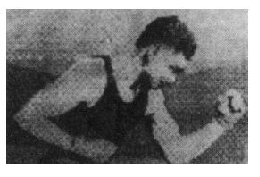
\includegraphics[scale=2]{capitulo_marcoteorico/dpiearly.pdf}
    \caption{Uno de los primeros ejemplos de imagen digital}\label{fig:dpiearly}
\end{figure}

Fue hasta 1960 que las computadoras tuvieron suficiente poder computacional para
manipular imágenes de manera efectiva. Las primeras aplicaciones estaban
relacionadas con sondas espaciales, para mejorar la calidad de las imágenes
tomadas por la NASA. Teniendo aplicación directa en la mejora de imágenes
capturadas de la superficial lunar.

En paralelo a estas aplicaciones y en 1970, se comenzó en la investigación de
imágenes digitales, su procesamiento y posterior aplicación al área médica, tema
que trata esta tesis. En esta década fue cuando se inventó la Tomografía Axial
Computarizada, uno de los mayores avances en la tecnología médica y que permitía
detectar tumores con precisión sin precedentes. La tomografía combina imágenes
como rebanadas para construir, mediante procesamiento digital de imágenes, una
representación en tres dimensiones del objeto.

Las aplicaciones actuales del procesamiento digital de imágenes existen en todo
el espectro de la actividad humana. Desde procesamiento de imágenes biológicas,
de geología, climatología, agricultura, arte digital, diseño gráfico,
publicidad, industria y entretenimiento. Es ahora cuando podemos encontrar
poderosos algoritmos en dispositivos móviles, lo cual ha incrementado el
contacto de la gente con esta técnica.

Otras áreas como los gráficos computacionales, las matemáticas, las artes y el
entretenimiento han incidido positivamente en el desarrollo de las imágenes
digitales y su procesamiento. Concretamente, las artes y el entretenimiento han
generado un interés generalizado en el área~\cite{Gonzalez2001}.

\subsubsection{Métodos}

Una imagen \index{Imagen digital} es una función \(f(x,y)\) donde \(x\) e \(y\)
son coordenadas espaciales planas. El valor de \(f(x)\) evaluado en cualquier
punto es la intensidad del pixel en esas coordenadas. Un pixel (acrónimo de
\emph{picture element}) es el mínimo componente de una imagen y corresponde a un
valor numérico. En RGB corresponde a los valores de intensidad que se encuentran
entre 0 y 255, intensidad se refiere a la fuerza de los fotones en ese punto en
específico (\autoref{fig:imagenarray}).

\begin{figure}[H]
    \centering
    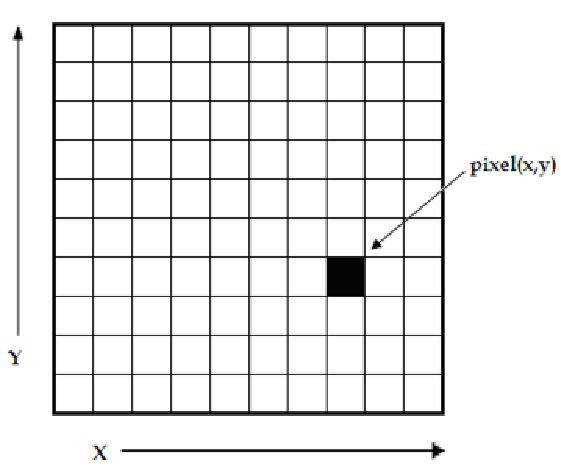
\includegraphics[width=0.5\textwidth]{capitulo_marcoteorico/imagen_array.pdf}
    \caption{Imagen como función (escala de grises)}\label{fig:imagenarray}
\end{figure}

Como podemos ver, las imágenes son naturalmente representadas por arreglos
rectangulares de números, es decir, matrices. Donde cada elemento de la matriz
representa la intensidad del pixel en esa posición. Es decir, una matrix de \(20
\times 20\) representa una imagen de \(20 \times 20\) pixeles de resolución. Es
por esta razón que el Álgebra Lineal es la rama de las matemáticas que rige el
comportamiento de las imágenes y es la razón por la cual la acción de manipular
una imagen matricial es optimizable mediante procesadores especializados en
gráficos..

\subsubsection{Espacios de color}

Una matriz de \(n \times n\) solo es capaz de representar una imagen en escala
de grises y debido a ello se requiere de más información para poder generar una
imagen a color.

Una imagen a color es un \emph{Tensor}, es decir, un arreglo de matrices \(m
\times n \times d\), donde \(m \times n\) es el tamaño de la imagen y \(d\) es
la matriz que representa el componente de color de cada imagen. Dependiendo del
espacio de color, este componente puede variar.

Un espacio de color es una abstracción matemática de los colores y de la
representación de sus características en una imagen digital. Los principales
espacios de color y sus derivados son los siguientes:

\begin{enumerate}
    \item{\textbf{CIE:}} Los espacios de color LAB son un viejo estándar de
    1976. Donde los componentes de color son L para luminosidad y a, b para
    componentes verde-rojo y azul-amarillo respectivamente. Fue diseñado para
    estar en armonía con la visión humana, ya que permite la representación de
    infinitos colores.

    \item{\textbf{RGB:}} Red-Green-Blue (Rojo-Verde-Azul) y su variante BGR es
    un espacio aditivo de color cuyo propósito es la representación de imágenes
    en medios digitales como pantallas y monitores. Probablemente sea el espacio
    de color más usado en las ciencias de la computación y puede rastrear sus
    orígenes a 1861 con James Clerk Maxwell, también es el más usado para
    capturar y mostrar imágenes y video digital, por lo cual será usado en esta
    tesis (\autoref{fig:rgbspace}). 

    \begin{figure}[H]
        \centering
        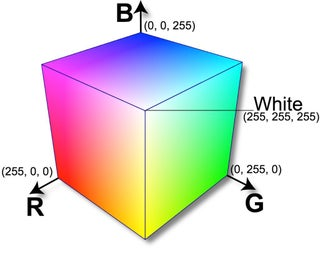
\includegraphics[width=0.5\textwidth]{capitulo_marcoteorico/rgb.jpg}
        \caption{RGB}\label{fig:rgbspace}
    \end{figure}

    \item{\textbf{Cilíndricos:}} HSV y HSL son dos modelos pensados para mejorar
    RGB y su representación con la visión humana. H es hue (tono), S es
    saturación, V es valor y L es luminosidad. Su geometría es cilíndrica.
\end{enumerate}

El uso del color convierte nuestra función inicial de recibir dos entradas a
tres: \(f(x,y,z)\) donde \(z\) es el eje tridimensional donde se encuentran los
componentes de color de alguno de los espacios aquí expuestos \cite{Vernon1991}.

\subsubsection{Manejo computacional de una imagen}

En resumen, una imagen es una matriz \(m \times n \times d\) definida por cierta
función \(f(x,y,z)\) donde cada elemento \(i-j~\acute{e}simo\) de tal matriz
representa la intensidad de un pixel dentro de una imagen de \(m \times n \)
pixeles. 

Es natural poder manipular estas imágenes mediante operaciones y funciones que
reciban matrices como entrada. La suma \(\mathbf{A} + \mathbf{B}\), resta
\(\mathbf{A} - \mathbf{B}\), producto cruz \(\mathbf{A} \times \mathbf{B}\),
producto punto \(\mathbf{A} \bullet \mathbf{B}\),  producto de Hadamard
\(\mathbf{A} \circ \mathbf{B}\), el producto de Kronecker \(\mathbf{A} \otimes
\mathbf{B}\) y producto escalar \(a \cdot \mathbf{A}\) son algunas operaciones
definidas para las matrices y que se usan en el procesamiento digital de
imágenes. Así como otras operaciones vectoriales, escalares, estadísticas,
trigonométricas y geométricas.

La representación matricial de las imágenes también nos permite realizar
operaciones que no serían naturales dentro de nuestro ambiente tridimensional.
Podemos generar imágenes no solo con un arreglo tensorial en forma de cuadrado o
cubo, sino podemos trabajar \(n-dimensionalmente\) donde cada canal puede
representar los tres componentes de color pero también representar datos
volumétricos en las dimensiones subsecuentes u otros espectros de color, esto es
muy común en el área médica, como en los archivos generados por las máquinas de
imagenología (\autoref{fig:ndimarray}) \cite{Toennies2012}. 

\begin{figure}[H]
    \centering
    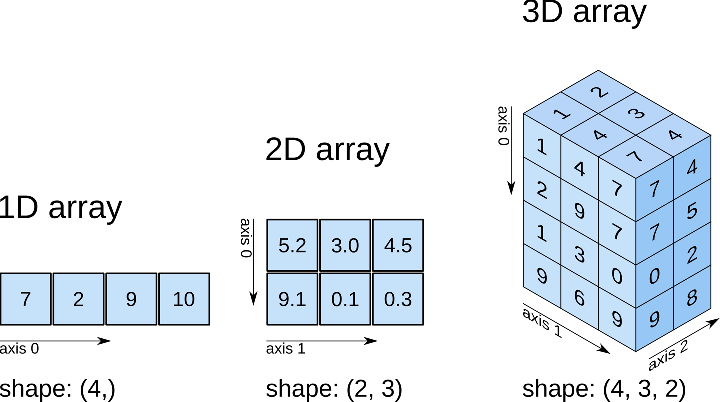
\includegraphics[width=0.5\textwidth]{capitulo_marcoteorico/ndimarray.pdf}
    \caption{Arreglos n dimensionales y su representación gráfica con el módulo Numpy}\label{fig:ndimarray}
\end{figure}

\subsubsection{Captura de imagen}

Aparte del tratamiento matemático de una imagen, el \hyperlink{abbr}{PDI}
también se encarga del proceso que deriva en una imagen matricial. Dentro de la
cámara, se encarga de convertir el impacto de los fotones de luz en energía
eléctrica que posteriormente será codificada y transmitida al procesador que la
manipulará. Este proceso está automatizado totalmente mediante el software que
compone la mayoría de los dispositivos electrónicos disponibles para el
consumidor: computadoras personales, laptops, teléfonos inteligentes.

Gracias a esto, nos podemos enfocar únicamente en la creación de un software que
funja como interface entre la cámara y la \hyperlink{abbr}{ConvNet} ya
entrenada. Igualmente tiene que proveer la interface gráfica para la interacción
entre el usuario y el programa de software. No existe diferencia técnica en la
manipulación de imágenes discretas o video, ya que el video es solo una sucesión
rápida de imágenes individuales, aunque si llegará a consumir más recursos
computacionales.

El proceso de convertir una imagen análoga en una matriz numérica involucra dos
procesos (\autoref{fig:camara}) \cite{Gries2010}:

\begin{itemize}
    \item{\textbf{Analógico:}} Los fotones que rebotan en la superficie del
    objeto a capturar ingresan al lente de la cámara el cual amplifica o enfoca
    la señal luminosa y la transfiere a una serie de filtros para posteriormente
    pasar por un circuito llamado Convertidor Analógico-Digital.
    \item{\textbf{Digital:}} Una vez convertida a una señal digital, se
    transmite a circuitos que utilizan algoritmos de DPI escritos en lenguajes
    de muy bajo nivel para maximizar su rendimiento. La salida de este proceso
    es un archivo de imagen como .jpg o .png, etcétera.
\end{itemize}

\begin{figure}[H]
    \centering
    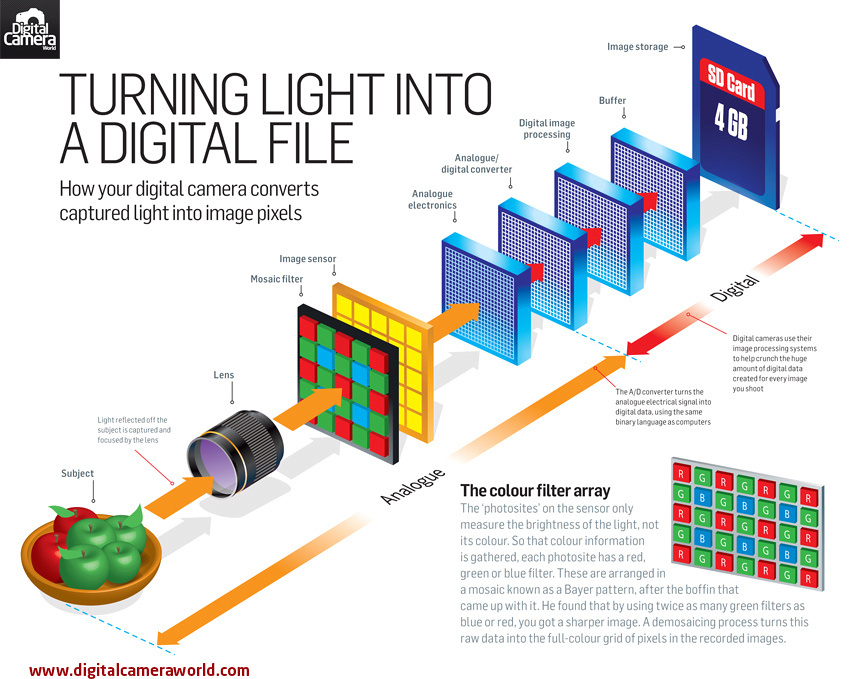
\includegraphics[width=0.7\textwidth]{capitulo_marcoteorico/camara.jpg}
    \caption{Esquema de una cámara digital}\label{fig:camara}
\end{figure}

En aplicaciones médicas, las imágenes no se limitan a aquellas que pueden ser
tomadas por cámaras tradicionales, sino también se usan otros dispositivos que
no necesariamente necesitan capturar imágenes en el espectro visible o usando
luz siquiera. Se pueden usar rayos X, resonancias magnéticas, tomografías o
ultrasonidos.

% \subsection{Algoritmos aplicados a imágenes}

% \subsubsection{Manipulación morfológica}

\subsection{Machine Learning}

Se define como la capacidad de hacer a las computadoras aprender de los datos,
sin ser explícitamente programadas para ello. Una definición técnica puede ser
la siguiente: 'Un programa de computadora se dice que aprende de la experiencia
$ E $, con respecto a alguna tarea $ T $ y alguna métrica de rendimiento $ P $;
si su rendimiento en $ T $, medido por $ P $, mejora con la experiencia $ E $'
\cite{Mitchell1997}.

La diferencia entre el modo tradicional de crear modelos inteligentes (como
aquellos basados en reglas) y hacer el uso del \hyperlink{abbr}{ML} se muestran
a continuación (\autoref{fig:tradicional} y \autoref{fig:moderna}). La
diferencia radica en la inclusión de una \hyperlink{abbr}{BD} y cambiar la fase
de escribir reglas (que es compleja, difícil y cara) por el entrenamiento del
algoritmo.

\tikzset{every picture/.style={line width=0.75pt}} %set default line width to 0.75pt        
\begin{figure}[H]
    \centering
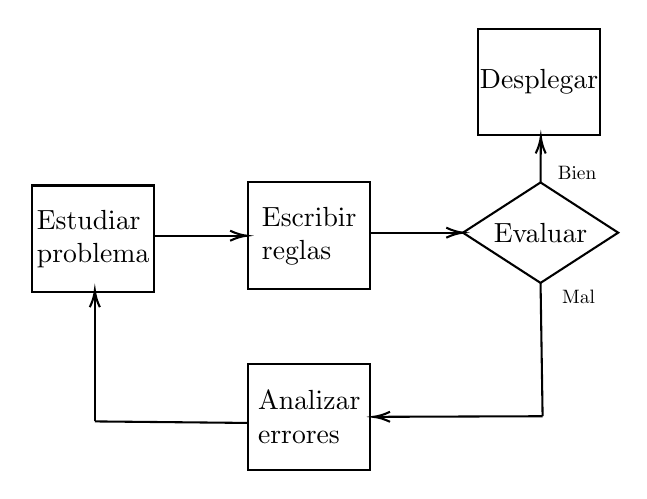
\begin{tikzpicture}[x=0.55pt,y=0.55pt,yscale=-1,xscale=1]
%uncomment if require: \path (0,300); %set diagram left start at 0, and has height of 300

%Flowchart: Process [id:dp1553966863793932] 
\draw   (58,107) -- (138,107) -- (138,177) -- (58,177) -- cycle ;
%Flowchart: Process [id:dp10248298188128446] 
\draw   (351,4) -- (431,4) -- (431,74) -- (351,74) -- cycle ;
%Flowchart: Decision [id:dp9521517530969476] 
\draw   (392,105) -- (443,138) -- (392,171) -- (341,138) -- cycle ;
%Straight Lines [id:da28478730888988457] 
\draw    (138,140) -- (197,140) ;
\draw [shift={(199,140)}, rotate = 180] [color={rgb, 255:red, 0; green, 0; blue, 0 }  ][line width=0.75]    (10.93,-3.29) .. controls (6.95,-1.4) and (3.31,-0.3) .. (0,0) .. controls (3.31,0.3) and (6.95,1.4) .. (10.93,3.29)   ;

%Flowchart: Process [id:dp08944572839701259] 
\draw   (200,105) -- (280,105) -- (280,175) -- (200,175) -- cycle ;
%Straight Lines [id:da26098363220700604] 
\draw    (280,138) -- (339,138) ;
\draw [shift={(341,138)}, rotate = 180] [color={rgb, 255:red, 0; green, 0; blue, 0 }  ][line width=0.75]    (10.93,-3.29) .. controls (6.95,-1.4) and (3.31,-0.3) .. (0,0) .. controls (3.31,0.3) and (6.95,1.4) .. (10.93,3.29)   ;

%Flowchart: Process [id:dp9395738678043528] 
\draw   (200,224) -- (280,224) -- (280,294) -- (200,294) -- cycle ;
%Straight Lines [id:da14493819086985438] 
\draw    (392,105) -- (392.16,77) ;
\draw [shift={(392.17,75)}, rotate = 450.32] [color={rgb, 255:red, 0; green, 0; blue, 0 }  ][line width=0.75]    (10.93,-3.29) .. controls (6.95,-1.4) and (3.31,-0.3) .. (0,0) .. controls (3.31,0.3) and (6.95,1.4) .. (10.93,3.29)   ;

%Straight Lines [id:da3456694459786809] 
\draw    (392,171) -- (393.35,258.6) ;


%Straight Lines [id:da17977075900916983] 
\draw    (393.35,258.6) -- (284.17,258.99) ;
\draw [shift={(282.17,259)}, rotate = 359.78999999999996] [color={rgb, 255:red, 0; green, 0; blue, 0 }  ][line width=0.75]    (10.93,-3.29) .. controls (6.95,-1.4) and (3.31,-0.3) .. (0,0) .. controls (3.31,0.3) and (6.95,1.4) .. (10.93,3.29)   ;

%Straight Lines [id:da4338896417108612] 
\draw    (99.17,262) -- (199.17,263) ;


%Straight Lines [id:da5774229996167787] 
\draw    (99.17,262) -- (99.17,178) ;
\draw [shift={(99.17,176)}, rotate = 450] [color={rgb, 255:red, 0; green, 0; blue, 0 }  ][line width=0.75]    (10.93,-3.29) .. controls (6.95,-1.4) and (3.31,-0.3) .. (0,0) .. controls (3.31,0.3) and (6.95,1.4) .. (10.93,3.29)   ;


% Text Node
\draw (98,142) node  [align=left] {Estudiar\\problema};
% Text Node
\draw (240,140) node  [align=left] {Escribir \\reglas};
% Text Node
\draw (392,138) node  [align=left] {Evaluar};
% Text Node
\draw (391,39) node  [align=left] {Desplegar};
% Text Node
\draw (240,259) node  [align=left] {Analizar\\errores};
% Text Node
\draw (416,99) node [scale=0.7] [align=left] {Bien};
% Text Node
\draw (417,180) node [scale=0.7] [align=left] {Mal};

\end{tikzpicture}
\caption{Metodología tradicional para crear un sistema inteligente}
\label{fig:tradicional}
\end{figure}

\begin{figure}[H]
    \centering
\tikzset{every picture/.style={line width=0.75pt}} %set default line width to 0.75pt        

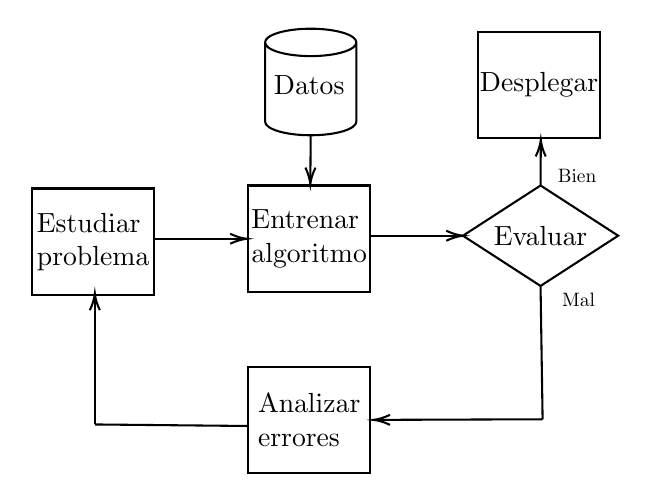
\begin{tikzpicture}[x=0.55pt,y=0.55pt,yscale=-1,xscale=1]
%uncomment if require: \path (0,300); %set diagram left start at 0, and has height of 300

%Flowchart: Process [id:dp1553966863793932] 
\draw   (58,107) -- (138,107) -- (138,177) -- (58,177) -- cycle ;
%Flowchart: Process [id:dp10248298188128446] 
\draw   (351,4) -- (431,4) -- (431,74) -- (351,74) -- cycle ;
%Flowchart: Decision [id:dp9521517530969476] 
\draw   (392,105) -- (443,138) -- (392,171) -- (341,138) -- cycle ;
%Straight Lines [id:da28478730888988457] 
\draw    (138,140) -- (197,140) ;
\draw [shift={(199,140)}, rotate = 180] [color={rgb, 255:red, 0; green, 0; blue, 0 }  ][line width=0.75]    (10.93,-3.29) .. controls (6.95,-1.4) and (3.31,-0.3) .. (0,0) .. controls (3.31,0.3) and (6.95,1.4) .. (10.93,3.29)   ;

%Flowchart: Process [id:dp08944572839701259] 
\draw   (200,105) -- (280,105) -- (280,175) -- (200,175) -- cycle ;
%Straight Lines [id:da26098363220700604] 
\draw    (280,138) -- (339,138) ;
\draw [shift={(341,138)}, rotate = 180] [color={rgb, 255:red, 0; green, 0; blue, 0 }  ][line width=0.75]    (10.93,-3.29) .. controls (6.95,-1.4) and (3.31,-0.3) .. (0,0) .. controls (3.31,0.3) and (6.95,1.4) .. (10.93,3.29)   ;

%Flowchart: Process [id:dp9395738678043528] 
\draw   (200,224) -- (280,224) -- (280,294) -- (200,294) -- cycle ;
%Straight Lines [id:da14493819086985438] 
\draw    (392,105) -- (392.16,77) ;
\draw [shift={(392.17,75)}, rotate = 450.32] [color={rgb, 255:red, 0; green, 0; blue, 0 }  ][line width=0.75]    (10.93,-3.29) .. controls (6.95,-1.4) and (3.31,-0.3) .. (0,0) .. controls (3.31,0.3) and (6.95,1.4) .. (10.93,3.29)   ;

%Straight Lines [id:da3456694459786809] 
\draw    (392,171) -- (393.35,258.6) ;


%Straight Lines [id:da17977075900916983] 
\draw    (393.35,258.6) -- (284.17,258.99) ;
\draw [shift={(282.17,259)}, rotate = 359.78999999999996] [color={rgb, 255:red, 0; green, 0; blue, 0 }  ][line width=0.75]    (10.93,-3.29) .. controls (6.95,-1.4) and (3.31,-0.3) .. (0,0) .. controls (3.31,0.3) and (6.95,1.4) .. (10.93,3.29)   ;

%Straight Lines [id:da4338896417108612] 
\draw    (99.17,262) -- (199.17,263) ;


%Straight Lines [id:da5774229996167787] 
\draw    (99.17,262) -- (99.17,178) ;
\draw [shift={(99.17,176)}, rotate = 450] [color={rgb, 255:red, 0; green, 0; blue, 0 }  ][line width=0.75]    (10.93,-3.29) .. controls (6.95,-1.4) and (3.31,-0.3) .. (0,0) .. controls (3.31,0.3) and (6.95,1.4) .. (10.93,3.29)   ;

%Shape: Can [id:dp13652945783356163] 
\draw   (271,11) -- (271,63) .. controls (271,67.97) and (257.57,72) .. (241,72) .. controls (224.43,72) and (211,67.97) .. (211,63) -- (211,11)(271,11) .. controls (271,15.97) and (257.57,20) .. (241,20) .. controls (224.43,20) and (211,15.97) .. (211,11) .. controls (211,6.03) and (224.43,2) .. (241,2) .. controls (257.57,2) and (271,6.03) .. (271,11) -- cycle ;
%Straight Lines [id:da8312712836328588] 
\draw    (241,72) -- (240.75,102.2) ;
\draw [shift={(240.73,104.2)}, rotate = 270.47] [color={rgb, 255:red, 0; green, 0; blue, 0 }  ][line width=0.75]    (10.93,-3.29) .. controls (6.95,-1.4) and (3.31,-0.3) .. (0,0) .. controls (3.31,0.3) and (6.95,1.4) .. (10.93,3.29)   ;


% Text Node
\draw (98,142) node  [align=left] {Estudiar\\problema};
% Text Node
\draw (240,140) node  [align=left] {Entrenar\\algoritmo};
% Text Node
\draw (392,138) node  [align=left] {Evaluar};
% Text Node
\draw (391,39) node  [align=left] {Desplegar};
% Text Node
\draw (240,259) node  [align=left] {Analizar\\errores};
% Text Node
\draw (416,99) node [scale=0.7] [align=left] {Bien};
% Text Node
\draw (417,180) node [scale=0.7] [align=left] {Mal};
% Text Node
\draw (240,39) node  [align=left] {Datos};


\end{tikzpicture}
\caption{Metodología de Machine Learning para crear un sistema inteligente}
\label{fig:moderna}
\end{figure}

\subsubsection{Fases del Machine Learning}

Hay cuatro fases básicas en cualquier forma de implementación de
\hyperlink{abbr}{ML} a cualquier dominio (\autoref{fig:machine}, para el
problema de clasificar imágenes entre perros y gatos) \cite{Watt2016}:

\begin{itemize}
    \item{\textbf{Recolectar datos:}} El algoritmo debe ser entrenado para poder
    realizar su función mediante la alimentación de lotes de imágenes en la fase
    de entrenamiento. Una \hyperlink{abbr}{BD} grande y diversa generará un
    mejor aprendizaje ya que proveerá al algoritmo de mayor experiencia.
    \item{\textbf{Diseño de características:}} Es en esta fase donde se aplica
    la ingeniería y extracción de las características representativas del
    problema a resolver y que maximizarán el rendimiento de un algoritmo. La
    ingeniería de características depende de muchísimo conocimiento del dominio
    específico de aplicación del algoritmo, generalmente en la forma de expertos
    mientras que para extraer las características, en el caso de las imágenes se
    pensará en color, tamaño, forma y proporción para constituir como los
    criterios de decisión para clasificar tal imagen, el cual requerirá un
    procesamiento previo con algoritmos de \hyperlink{abbr}{PDI}. Este proceso
    también es complejo y difícil (aunque mucho menos que diseñar reglas
    \emph{ad hoc} para cada aplicación) y requiere de métodos auxiliares como el
    \hyperlink{abbr}{PDI} o, en caso de datos tabulares, mucha estadística.
    \item{\textbf{Entrenamiento del modelo:}} En los problemas de clasificación,
    entrenar un modelo se reduce a encontrar una interpretación geométrica del
    espacio de las características que pueda ser separada mediante una línea
    recta (en caso de sistemas lineales), que servirá como frontera entre cada
    clase. Entrenamiento se refiere a buscar los parámetros que regirán el
    comportamiento de esta frontera para clasificar correctamente las imágenes.
    \item{\textbf{Prueba del modelo:}} Una vez entrenado, se requiere probar la
    eficacia del modelo mediante la alimentación del mismo con un conjunto de
    imágenes que no hayan sido vistas nunca por el algoritmo. Esto medirá el
    poder de generalización y nos permitirá evaluar, dado su rendimiento, si
    este es aceptable o se requieren diagnosticar problemas en la implementación
    del modelo (como una \hyperlink{abbr}{BD} muy pequeña). 
\end{itemize}

\begin{figure}[H]
    \centering
    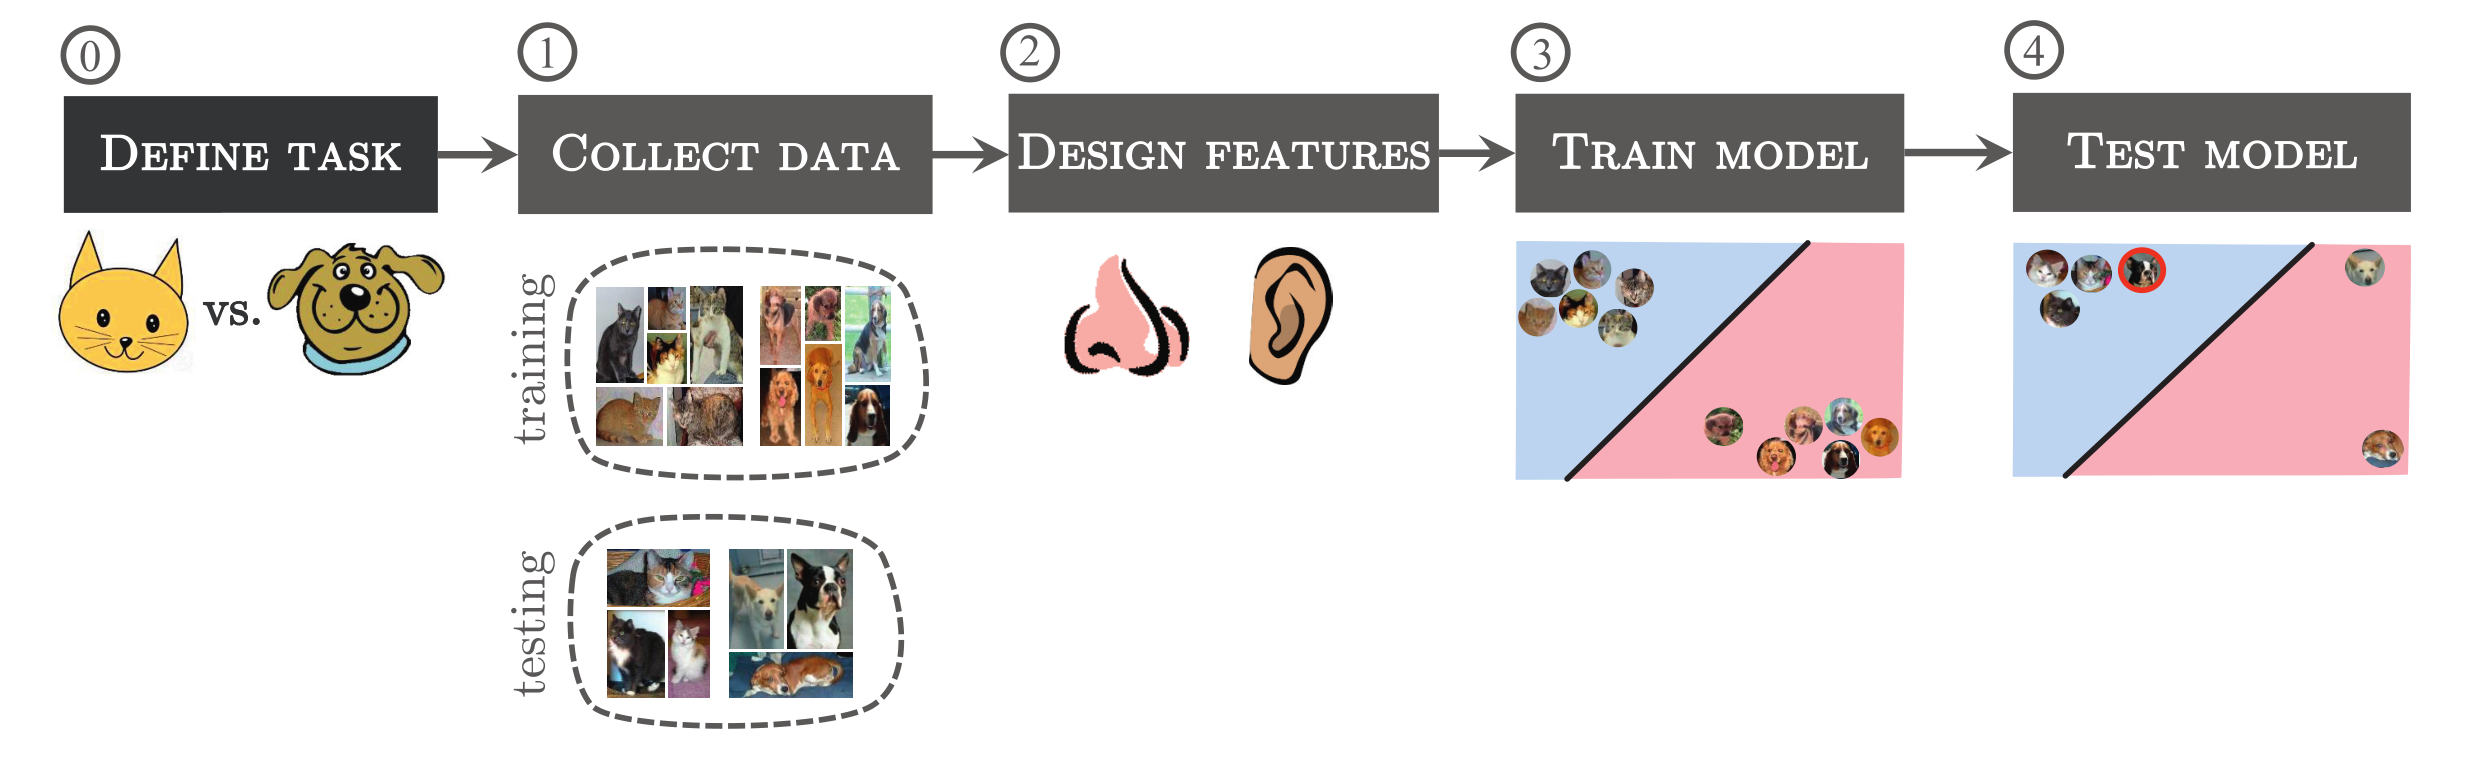
\includegraphics[width=0.9\textwidth]{capitulo_marcoteorico/machine}
    \caption{Fases básicas del Machine Learning}\label{fig:machine}
\end{figure}

Las tres cosas mínimas requeridas para hacer \hyperlink{abbr}{ML} son:

\begin{enumerate}
    \item{Datos de entrada}
    \item{Las etiquetas de salida}
    \item{Una métrica de error} 
\end{enumerate}

El \hyperlink{abbr}{ML} nos permite no solo cambiar pasos dentro de una
metodología para crear sistemas inteligentes, sino también nos otorga de un
paradigma distinto de pensamiento. Antes necesitamos generar una serie de reglas
y combinarlas con datos para tener respuestas, ahora, necesitamos datos y
respuestas para poder obtener reglas (\autoref{fig:paradigma})
\cite{Chollet2018}.

\tikzset{every picture/.style={line width=0.75pt}} %set default line width to 0.75pt        
\begin{figure}[H]
    \centering  

    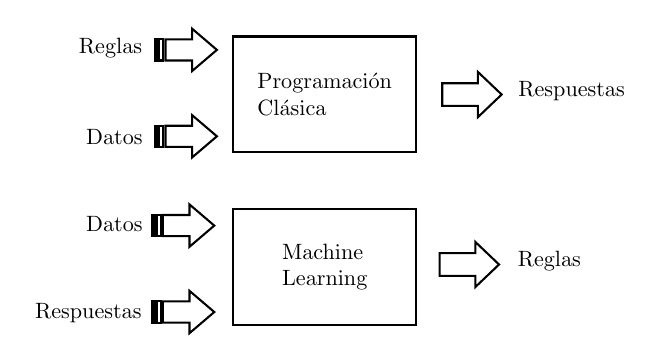
\begin{tikzpicture}[x=0.75pt,y=0.75pt,yscale=-1,xscale=1]
    %uncomment if require: \path (0,300); %set diagram left start at 0, and has height of 300
    
    %Shape: Rectangle [id:dp5656002629863663] 
    \draw   (331.05,93.82) -- (419.15,93.82) -- (419.15,149.34) -- (331.05,149.34) -- cycle ;
    %Shape: Rectangle [id:dp08469876048021208] 
    \draw   (331.05,10.55) -- (419.15,10.55) -- (419.15,66.06) -- (331.05,66.06) -- cycle ;
    %Right Arrow [id:dp5526832475614203] 
    \draw   (431.74,33.07) -- (448.91,33.07) -- (448.91,27.62) -- (460.35,38.51) -- (448.91,49.41) -- (448.91,43.96) -- (431.74,43.96) -- cycle ;
    %Right Arrow [id:dp11323285532946126] 
    \draw   (430.48,114.95) -- (447.65,114.95) -- (447.65,109.5) -- (459.09,120.4) -- (447.65,131.29) -- (447.65,125.85) -- (430.48,125.85) -- cycle ;
    %Striped Right Arrow [id:dp37446377869018366] 
    \draw   (298.39,11.9) -- (311.21,11.9) -- (311.21,6.8) -- (323.16,17) -- (311.21,27.2) -- (311.21,22.1) -- (298.39,22.1) -- cycle ;\draw   (293.29,11.9) -- (294.31,11.9) -- (294.31,22.1) -- (293.29,22.1) -- cycle ;\draw   (295.33,11.9) -- (297.37,11.9) -- (297.37,22.1) -- (295.33,22.1) -- cycle ;
    %Striped Right Arrow [id:dp511490599188687] 
    \draw   (298.39,53.54) -- (311.21,53.54) -- (311.21,48.44) -- (323.16,58.64) -- (311.21,68.84) -- (311.21,63.74) -- (298.39,63.74) -- cycle ;\draw   (293.29,53.54) -- (294.31,53.54) -- (294.31,63.74) -- (293.29,63.74) -- cycle ;\draw   (295.33,53.54) -- (297.37,53.54) -- (297.37,63.74) -- (295.33,63.74) -- cycle ;
    %Striped Right Arrow [id:dp24056201288099344] 
    \draw   (297.13,96.56) -- (309.95,96.56) -- (309.95,91.46) -- (321.9,101.66) -- (309.95,111.86) -- (309.95,106.76) -- (297.13,106.76) -- cycle ;\draw   (292.03,96.56) -- (293.05,96.56) -- (293.05,106.76) -- (292.03,106.76) -- cycle ;\draw   (294.07,96.56) -- (296.11,96.56) -- (296.11,106.76) -- (294.07,106.76) -- cycle ;
    %Striped Right Arrow [id:dp09567701368722925] 
    \draw   (297.13,138.2) -- (309.95,138.2) -- (309.95,133.1) -- (321.9,143.3) -- (309.95,153.5) -- (309.95,148.4) -- (297.13,148.4) -- cycle ;\draw   (292.03,138.2) -- (293.05,138.2) -- (293.05,148.4) -- (292.03,148.4) -- cycle ;\draw   (294.07,138.2) -- (296.11,138.2) -- (296.11,148.4) -- (294.07,148.4) -- cycle ;
    
    
    % Text Node
    \draw (375.1,38.31) node [scale=0.8] [align=left] {Programación\\Clásica};
    % Text Node
    \draw (375.1,121.58) node [scale=0.8] [align=left] {Machine\\Learning};
    % Text Node
    \draw (271.89,16.1) node [scale=0.8] [align=left] {Reglas};
    % Text Node
    \draw (483.34,118.8) node [scale=0.8] [align=left] {Reglas};
    % Text Node
    \draw (273.78,100.76) node [scale=0.8] [align=left] {Datos};
    % Text Node
    \draw (273.78,59.12) node [scale=0.8] [align=left] {Datos};
    % Text Node
    \draw (261.19,143.78) node [scale=0.8] [align=left] {Respuestas};
    % Text Node
    \draw (494.04,36.92) node [scale=0.8] [align=left] {Respuestas};
    
    
    \end{tikzpicture}
    
\caption{Un nuevo paradigma}
\label{fig:paradigma}
\end{figure}

\subsubsection{Tipos y algoritmos de Machine Learning}

Existen muchas formas de clasificar los algoritmos de \hyperlink{abbr}{ML},
algunos los clasifican por su forma de aprendizaje o la forma en la que realizan
sus generalizaciones. En este caso nos centraremos en la forma en que los
algoritmos aprenden, en referencia a la presencia o ausencia de respuestas para
alimentar la función de pérdida\cite{AurelienGeron2017}.

El \textbf{aprendizaje supervisado} es aquel que se alimenta con los datos de
entrenamiento en conjunto a las soluciones o \emph{labels} (etiquetas). Este
tipo de aprendizaje puedes resolver las tareas de clasificación y regresión.
Clasificar significa separar dos (clasificación binaria) o más (clasificación
multi-clase) conjuntos de entradas y asignarles una variable categórica.
Regresión es la predicción de un valor numérico continuo
(\autoref{fig:class_reg}).

\begin{figure}[H]
    \centering
    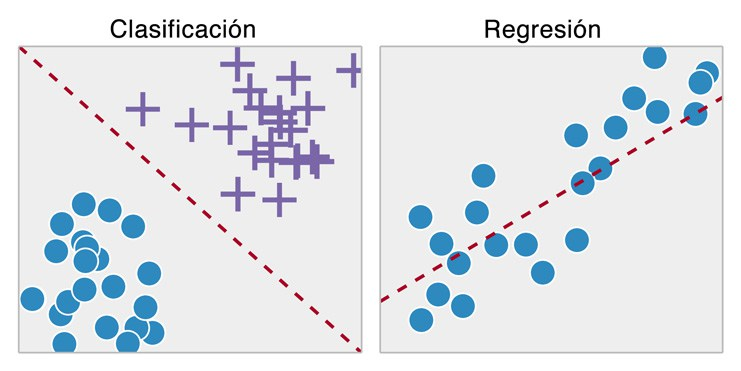
\includegraphics[width=0.5\textwidth]{capitulo_marcoteorico/clasificacion_regresion}
    \caption{Tareas del aprendizaje supervisado}\label{fig:class_reg}
\end{figure}

Algunos algoritmos de aprendizaje supervisado son los siguientes:

\begin{itemize}
    \item k-Nearest Neighbors
    \item Linear Regression
    \item Logistic Regression
    \item Support Vector Machines
    \item Decision Trees
    \item XGBoost
\end{itemize} 

El \textbf{aprendizaje no supervisado}, no requiere de etiquetas para su
funcionamiento. Es capaz de encontrar relaciones no explícitas entre los datos y
tiene las siguientes dos aplicaciones (\autoref{fig:cluster}):

\begin{figure}[H]
    \centering
    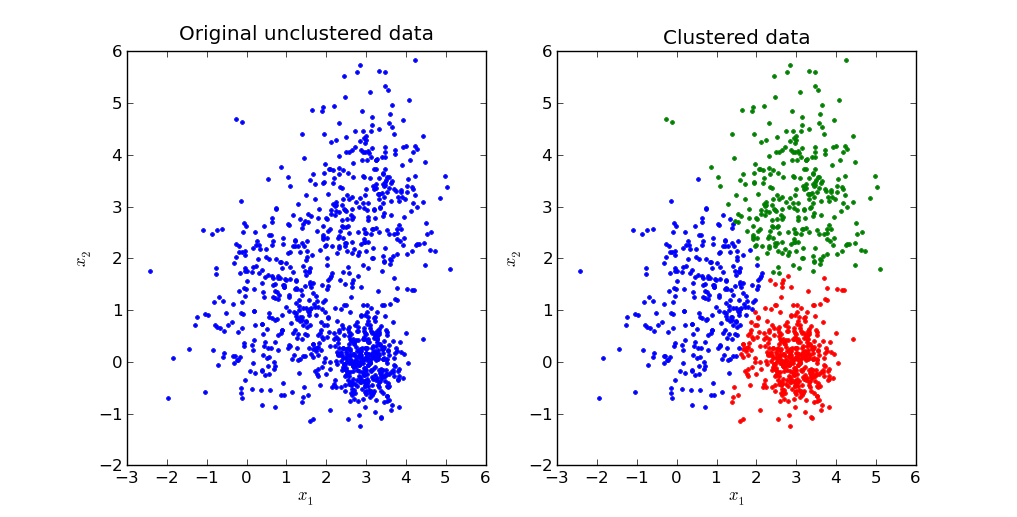
\includegraphics[width=0.7\textwidth]{capitulo_marcoteorico/cluster}
    \caption{Clustering}\label{fig:cluster}
\end{figure}

\begin{enumerate}
    \item Clustering
    \begin{itemize}
        \item k-Means
        \item Hierarchical Cluster Analysis (HCA)
        \item Expectation Maximization
    \end{itemize}
    \item Visualización y reducción de la dimensionalidad
    \begin{itemize}
        \item Principal Component Analysis (PCA)
        \item Self Organizing Maps
        \item t-distributed Stochastic Neighbor Embedding (\hyperlink{abbr}{t-SNE}\nomenclature{t-SNE}{t-distributed Stochastic Neighbor Embedding})
    \end{itemize}
\end{enumerate}

Tenemos muchísimos algoritmos para realizar la misma tarea que podríamos llegar
a pensar que existe una manera fácil o intuitiva para seleccionar el mejor de
todos para un problema dado. Lamentablemente el Teorema de no almuerzo gratis
(No Free Lunch) dice que no existe un modelo que funcione mejor para cada
problema. Es necesario hacer una búsqueda y probar todos los algoritmos que
nuestros recursos nos permitan. Es por ello que posteriormente haremos una
búsqueda entre todo el muchas arquitecturas neuronales distintas para encontrar
aquella que tenga el mejor rendimiento para el problema a resolver. 

El rendimiento de un algoritmo $a$ iterado $m$ veces bajo una función de pérdida
$f$ se mide con la probabilidad condicional de obtener una muestra particular
$d_{m}$ bajo las condiciones establecidas se muestra en la \autoref{Rendimiento
algorítmico}; donde $d^{y}_{m}$ representa las etiquetas de la muestra. 

\ecuacion{\Phi(d^{y}_{m}) = P(d^{y}_{m} | f, m ,a)}{Rendimiento algorítmico}

El teorema demuestra que si un algoritmo tiene un buen rendimiento en cierta
clase de problemas necesariamente tiene un rendimiento reducido en el resto
del conjunto de problemas. Esto se reduce a determinar como un subconjunto de
problemas perteneciente a todo el conjunto de problemas existentes $F_{1}
\subset \mathcal{F}$ para el cual el algoritmo $a_{1}$ tiene mejor rendimiento
que el algoritmo $a_{2}$ y compararlo con el subconjunto $F_{2} \subset
\mathcal{F}$ para el cual lo opuesto se cumple. Esto se logra sumando todas las
funciones de pérdida $f$ para $P(d^{y}_{m} | f, m ,a_{1})$ y comparándolas con
la suma de $P(d^{y}_{m} | f, m ,a_{2})$. La demostración del teorema conlleva al
resultado de que $P(d^{y}_{m} | f, m ,a)$ es independiente de $a$ cuando
promediamos sobre todas las funciones de pérdida (\autoref{Teorema
NFL})\cite{Wolpert1996}.

\ecuacion{\sum_{f} P(d^{y}_{m} | f, m, a_{1}) = \sum_{f} P( d^{y}_{m} | f, m, a_{2})}{Teorema NFL}

El único algoritmo de \hyperlink{abbr}{ML} que se usará dentro de esta tesis
será \hyperlink{abbr}{t-SNE}, que ayudará a visualizar el espacio altamente
dimensional del modelo de clasificación en dos dimensiones para ver como se
comporta. Este algoritmo funciona incrustando puntos de muchas dimensiones en
dimensiones bajas (generalmente dos) de cierta forma que se respete la similitud
entre puntos. Los cercanos en el espacio altamente dimensional corresponden a
los puntos cercanos incrustados en el espacio de dimensión reducida y viceversa
(\autoref{alg:tsne}) \cite{VanderMaaten2008}\cite{VanderMaaten2013}.

\begin{algorithm}[H]
    \SetAlgoLined
    \SetKwInOut{Input}{Input}\SetKwInOut{Output}{Output}
    \Input{data set $X = \{x_{1}, x_{2}, ..., x_{n}\}$}
    \BlankLine
    cost function parameters: perplexity \emph{Perp}
    \BlankLine
    optimization parameters: number of iterations $T$, learning rate $\eta$, momentum $\alpha(t)$.
    \BlankLine
    \Output{low-dimensional data representation $Y(T) = \{y_{1},y_{2}, ...,y_{n}\}$}
    \BlankLine
    \Begin{
        compute pairwise affinities $p_{j|i}$ with perplexity Perp
        \BlankLine
        $p_{j|i} \longleftarrow \frac{p_{j|i} + p_{i|j}}{2n}$
        \BlankLine
        sample initial solution $Y^{(0)} = \{y_{1},y_{2}, ...,y_{n}\}$  from $\mathcal{N}(0,10^{-4}I)$
        \BlankLine
        \For{$t = 1$ to $T$}{
            compute low-dimensional affinities $q_{ij}$
            \BlankLine
            compute gradient $\frac{\delta C}{\delta Y}$
            \BlankLine
            $Y^{(t)} \longleftarrow Y^{(t - 1)} + \eta \frac{\delta C}{\delta Y} + \alpha (t) (Y^{(t - 1)} - Y^{(t - 2))}$
        }

    }
    
    \caption{t-distributed Stochastic Neighbor Embedding}\label{alg:tsne}
    \end{algorithm}

\subsection{Selección de modelo}

El rendimiento de generalización de cualquier algoritmo de aprendizaje está
directamente relacionado con su capacidad de realizar predicciones correctas en
un subconjunto de datos especialmente separados para realizar pruebas al
algoritmo. La evaluación de este rendimiento es sumamente importante (más en la
práctica), ya que nos provee de una medida de la calidad de nuestro modelo. 

Para poder evaluar el rendimiento, debemos sobrepasar ciertas cuestiones
estadísticas como el dilema sesgo-varianza y algunos otros problemas
relacionados con el ajuste tanto del modelo como de los hiperparámetros.

Ajustar dichos hiperparámetros con los mismos datos usado para entrenar el
modelo, no se obtendrían buenos resultados ya que el modelo solo se dedicaría a
predecir sobre el mismo conjunto de datos, inhibiendo su capacidad de
generalización. Por lo tanto los hiperparámetros deben de ser ajustados con un
conjunto separados de datos sobre el cual el modelo aprenderá sus parámetros
internos (como los pesos en las redes neuronales). 

\subsubsection{Conjuntos de datos}

Como estamos hablando de aprendizaje supervisado, tenemos un conjunto de datos
correctamente etiquetado y se debe distribuir este recurso limitado para
entrenar, validar y probar el modelo. Claramente, usar el conjunto de datos
usado para aprender, como conjunto de evaluación, llevaría a una sobrestimación
del poder predictivo de nuestro modelo. Esto es porque, como hemos mencionado
anteriormente, la generalización es el objetivo primario, esto lo probamos
realizando predicciones sobre un conjunto que nuestro modelo jamás haya visto.
Así mismo, la porción de datos usados para la selección tanto del modelo (o
arquitectura) así como el ajuste de sus hiperparámetros también debe de ser
distinto. Fallar en esta fase llevaría a tener esperanzas demasiado optimistas
sobre el rendimiento del modelo, un fallo crítico si se trata del área
médica.~\cite{Learningb}

Dado cierto conjunto de datos \(\mathbb{D}\), tenemos los subconjuntos
\(\mathcal{T}, \mathcal{V}, \mathcal{P} \in \mathbb{D}\) Entrenamiento,
Validación y Prueba respectivamente, tal que:

\begin{itemize}
    \item{\textbf{Entrenamiento:}} Estos son los datos que serán usados para
    entrenar el modelo. Los mismos datos de entrenamiento servirán para probar
    distintos modelos y arquitecturas, lo que nos permite evaluar su rendimiento
    y seleccionar el mejor algoritmo para nuestro problema particular. 
    \item{\textbf{Validación:}} Estos datos son los que nos sirven para mejorar
    la precisión del modelo una vez que lo hayamos elegido, Estos datos nos
    permiten el ajuste de hiperparámetros, así como una evaluación primaria de
    nuestros modelos y nos otorga información para hacer cambios en los
    componentes de nuestras arquitecturas.
    \item{\textbf{Pruebas:}} Este subconjunto será utilizado para medir la
    precisión del modelo final. Es muy importante, que no se miren los datos
    durante el proceso y solamente usarlos al final; esto para no inducir ruido
    estadístico ni subjetividad. 
\end{itemize}    

\subsubsection{Estimación el error de generalización}

En la~\autoref{Categorical Crossentropy} notamos que, teniendo las etiquetas
correctas de cierta evaluación \(y\) como variable objetivo, un tensor de
entradas \(\mathsf{X}\) (en el caso de imágenes pueden ser en tanto en dos
dimensiones como volumétricas) y cierto modelo predictivo
\(\hat{f}(\mathsf{X})\) el cual hemos estimado en nuestro subconjunto de
entrenamiento \(\mathcal{T}\). La función de pérdida (Loss Function) que
cuantifica el error entre la etiqueta correcta Y y la predicha por el algoritmo
\(\hat{f}(\mathsf{X})\), para el caso de clasificación de imágenes se toma como
la función de pérdida \(L(y , \hat{f}(\mathsf{X}))\) la Entropía Cruzada (Cross
Entropy), tanto para clasificación binaria como multi-clase; mientras que el
Error Cuadrático Medio (MSE) es la función de pérdida usada para problemas de
regresión (\autoref{Mean Squared Error}) \cite{Hastie2009}.

% \begin{equation}
% \label{eq:loss}
% L(y , \hat{f}(\mathsf{X})) = {-(y\log(\hat{f}(\mathsf{X}))+(1-y)\log(1-\hat{f}(\mathsf{X})))}
% \end{equation}

\ecuacion{L(y , \hat{f}(\mathsf{X})) = - \frac{1}{N} \sum_{i=1}^{N} \log p_{\hat{f}(\mathsf{X})}[y_{i} \in C_{y_{i}}]}{Categorical Crossentropy}

% \begin{equation}
%     \label{eq:categorical}
%     L(y , \hat{f}(\mathsf{X})) = - \frac{1}{N} \sum_{i=1}^{N} \log p_{\hat{f}(\mathsf{X})}[y_{i} \in C_{y_{i}}] 
% \end{equation}

\ecuacion{L(y , \hat{f}(\mathsf{X}) = \frac{1}{n} \sum_{i=1}^{n}(y_{i} - \hat{f}(\mathsf{X_{i}}))^2}{Mean Squared Error}

% \begin{equation}
%     \label{eq:mse}
%     L(y , \hat{f}(\mathsf{X}) = \frac{1}{n} \sum_{i=1}^{n}(y_{i} - \hat{f}(\mathsf{X_{i}}))^2
% \end{equation}

Esta función de pérdida, es cierta medida del error que existe entre las
etiquetas reales y las predichas por el modelo. Por ende, el error que nos
interesa es el error de generalización, que está dado por la~\autoref{Error de
generalización}, donde el \(Err_{\mathcal{P}}\) es igual al valor esperado de
nuestra función de pérdida \(L(y , \hat{f}(\mathsf{X}))\) dato nuestro
subconjunto de prueba \(\mathcal{P}\).

\ecuacion{Err_{\mathcal{P}} = E[L(y , \hat{f}(\mathsf{X}))|\mathcal{P}]}{Error de generalización}

% \begin{equation}
%     \label{eq:error}
%     Err_{\mathcal{P}} = E[L(y , \hat{f}(\mathsf{X}))|\mathcal{P}]
%     \end{equation}

\subsubsection{Validación cruzada de K-iteraciones}

La división en estos tres conjuntos no siempre es posible ya que a veces
trabajamos con muy pocos datos, como en el área médica. Tener pocos datos
implica incertidumbre estadística en la estimación del error de generalización.
Otro problema que surge es que dividir los datos, si bien reducimos el sesgo,
podemos incidir ruido estadístico en el modelo, también entramos en errores de
redondeo, ya que los índices pertenecen al conjunto de los naturales \(i \in
\mathbb{N}\). Afortunadamente, la técnica de Validación Cruzada Iterativa
(K-fold Cross-Validation) soluciona ambos problemas, aunque no lo hace gratis,
sino que incurre en un costo computacional extra, lo cual lo hace poco práctico
cuando no se cuenta un equipo de cómputo adecuado.~\cite{Hastie2009}

La Validación Cruzada de K-Iteraciones (\autoref{alg:kfold}), es un algoritmo en
el cual cada partición del conjunto de datos \(\mathbb{D}\) se crea con
subconjuntos disjuntos del mismo. El error se estima en cada iteración del
algoritmo (\autoref{fig:kfold}).~\cite{Goodfellow2016}

\begin{figure}[H]
    \centering
    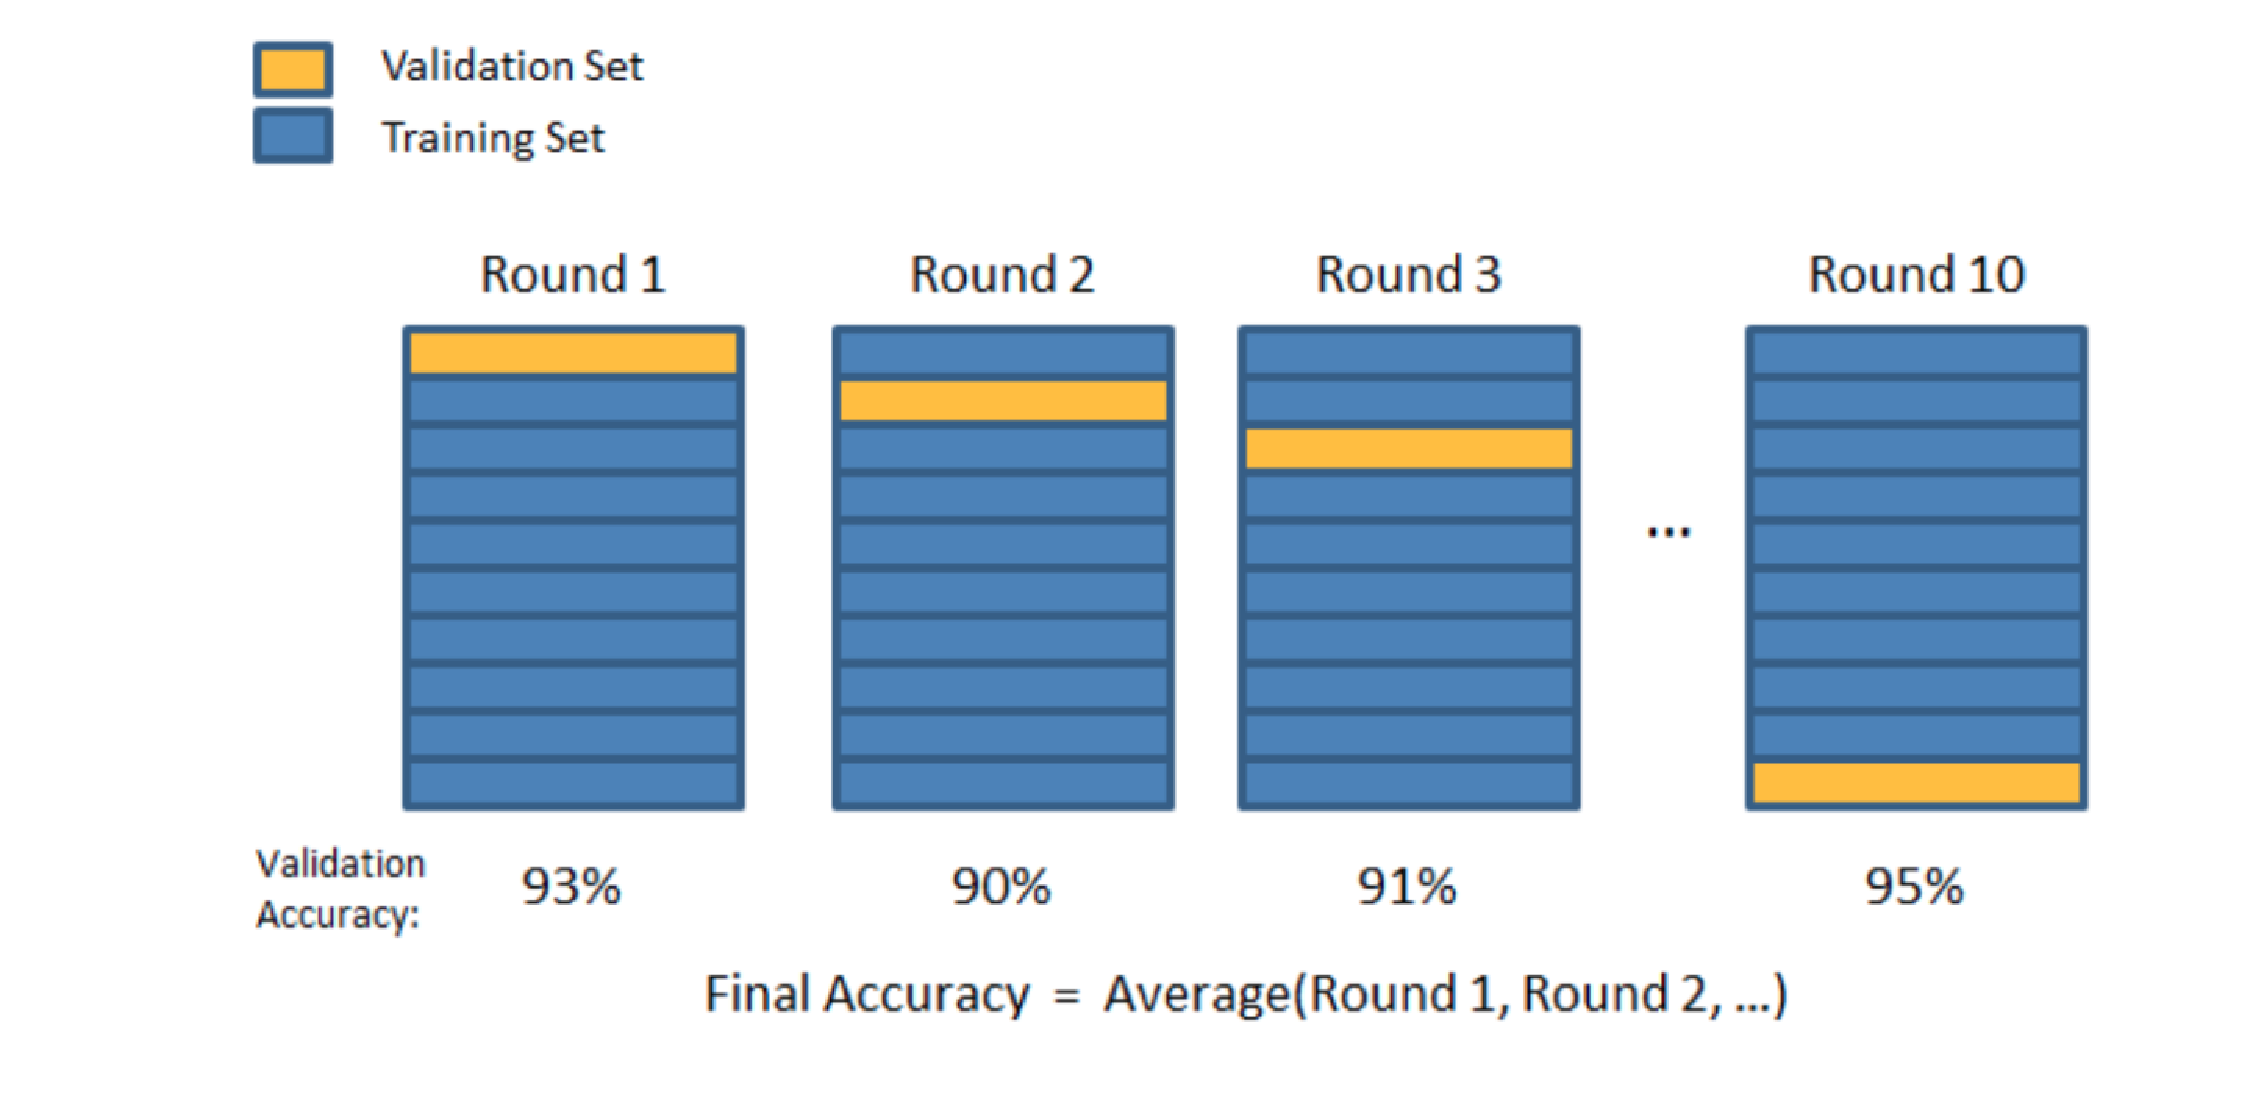
\includegraphics[scale=0.3]{capitulo_marcoteorico/cross.pdf}
    \caption{Ejemplo de Validación Cruzada}\label{fig:kfold}
\end{figure}

\begin{algorithm}[H]
    \SetAlgoLined
    \SetKwInOut{Input}{Input}\SetKwInOut{Output}{Output}
    \Input{Training set $ S = \{(\boldsymbol{\mathrm{x}}_{1}, y_{1}), ... , (\boldsymbol{\mathrm{x}}_{m}, y_{m})\} $}
    \BlankLine
    \Input{Parameters $ \Theta $}
    \BlankLine
    \Input{Algorithm $ A $}
    \BlankLine
    \Input{Folds $ k $}
    \BlankLine
    \Output{$ \theta^{*} = argmin_{\theta} [error(\theta)] $}
    \BlankLine
    \Output{$ h_{\theta^{*}} = A(S; \theta^{*}) $}
    \BlankLine
    \Begin{
        Divide $ S_{1}, S_{1}, ..., S_{k} \in S $
        \BlankLine
        \For{$ \theta $ in $ \Theta $}{
            \BlankLine
            \For{$ i = 1 $ to $ k $}{
                $ h_{i, \theta^{*}} \longleftarrow A(S \setminus S_{i}; \theta^{*}) $
                \BlankLine
                $ error(\theta) \longleftarrow \frac{1}{k} \sum_{i=1}^{k} L_{S_{i}} (h_{i, \theta^{*}}) $
            }
        }
    }
    \caption{Validación cruzada de K-iteraciones}\label{alg:kfold}
\end{algorithm}


Aunque existen otras formas de probar el modelo para encontrar el óptimo entre
el sesgo y la varianza, nos enfocamos solamente en la técnica de validación
cruzada. Ya que se ha encontrado que, en el área médica, es la mejor valida
estadísticamente el rendimiento de un modelo.~\cite{Ambroise2002}

\subsubsection{Sesgo contra varianza}

La mayoría de los modelos suponen relaciones funcionales entre las variables, lo
cual permite al modelo hacer un estimado de la variable objetivo en el caso del
aprendizaje supervisado. No todos los modelos hacen las mismas suposiciones, es
por ello que se requiere escoger las mejores para determinada
\hyperlink{abbr}{BD}.

Existen dos tipos de error en los modelos:

\begin{itemize}
    \item{\textbf{Sesgo: }} Es la diferencia entre el valor estimado y el valor
    verdadero de una variable. Son los errores derivados de las suposiciones
    incorrectas que hace el algoritmo o por un mal diseño de la
    \hyperlink{abbr}{BD}. Puede causar que un algoritmo identifique
    incorrectamente o pierda relaciones importantes, lo que puede resultar en
    \emph{underfitting} \index{Underfitting} o infra-ajuste; el modelo es
    incapaz de capturar el verdadero patrón subyacente dentro de la
    \hyperlink{abbr}{BD}
    \item{\textbf{Varianza: }} Es el error causado por la sensibilidad a
    pequeñas variaciones dentro de la \hyperlink{abbr}{BD} y es que tanto un
    estimado, dado cierto punto de dato, de cuanto cambiará este usando una
    \hyperlink{abbr}{BD} distinta. Una alta varianza puede hacer que el
    algoritmo realice sus estimaciones usando el ruido aleatorio en lugar de las
    relaciones en los datos. También está asociada al fenómeno de \emph{overfitting}
    \index{Overfitting} o sobre-ajuste, en el cual un algoritmo tiene un
    excelente rendimiento en el conjunto de entrenamiento pero tiene un poder de
    generalización muy pobre.
\end{itemize}

\subsubsection{Sobre-ajuste contra infra-ajuste}

Estos son dos conceptos están relacionados con el hecho de que los datos usados
para entrenar el modelo no son los datos con los que será implementado
(\autoref{fig:underfit}). 

\begin{figure}[H]
    \centering
    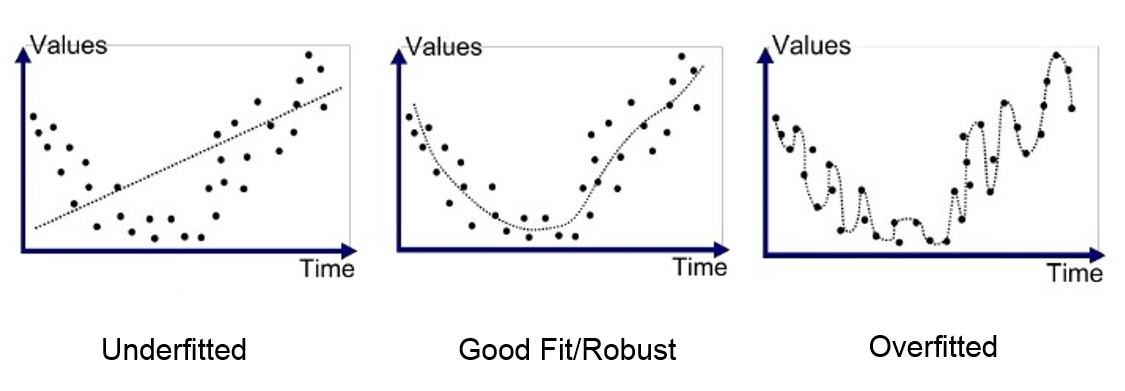
\includegraphics[width=0.8\textwidth]{capitulo_marcoteorico/underfit}
    \caption{Infra-ajuste vs sobre-ajuste vs buen ajuste}\label{fig:underfit}
\end{figure}


El \emph{underfitting} causa paupérrimas predicciones ya que el modelo no tiene
poder suficiente para capturar los patrones y relaciones que yacen en los datos.
Puede ser solucionado usando un otro algoritmo u otro modelo más complejo,
también se usan técnicas de regularización para evitarlo.

El \emph{overfitting} conlleva a predicciones excesivamente ajustadas a los
datos de entrenamiento. El modelo no aprendió de los datos, los memorizó. Esto
es asociado a una alta varianza y tienen un poder de generalización muy pobre.
Soluciones incluyen simplificar el modelo, obtener más datos de entrenamiento o
aplicar regularización.

Los modelos con baja varianza tienden a ser menos complejos, es decir, tienen
una estructura subyacente simple. Tienden a ser consistentes pero poco exactos.
Dependiendo de la \hyperlink{abbr}{BD}, pueden no ser suficientemente complejos
para encontrar el verdadero patrón, resultando en infra-ajuste.

Los modelos con sesgo bajo, son más complejos y son más flexibles en su
estructura interna; lo que permite más poder para encontrar relaciones complejas
dentro de los datos. Pueden llevar al sobre-ajuste ya que son tan poderosos que
pueden memorizar los datos en lugar de aprender de ellos. 

En la \autoref{fig:biasvvariance} podemos ver una analogía de estos dos tipos de
error. En el que cada punto representa no un dato, sino una iteración de
entrenamiento de cierto modelo, ajustado al mismo problema utilizando distintas
\hyperlink{abbr}{BD}s.

\begin{figure}[H]
    \centering
    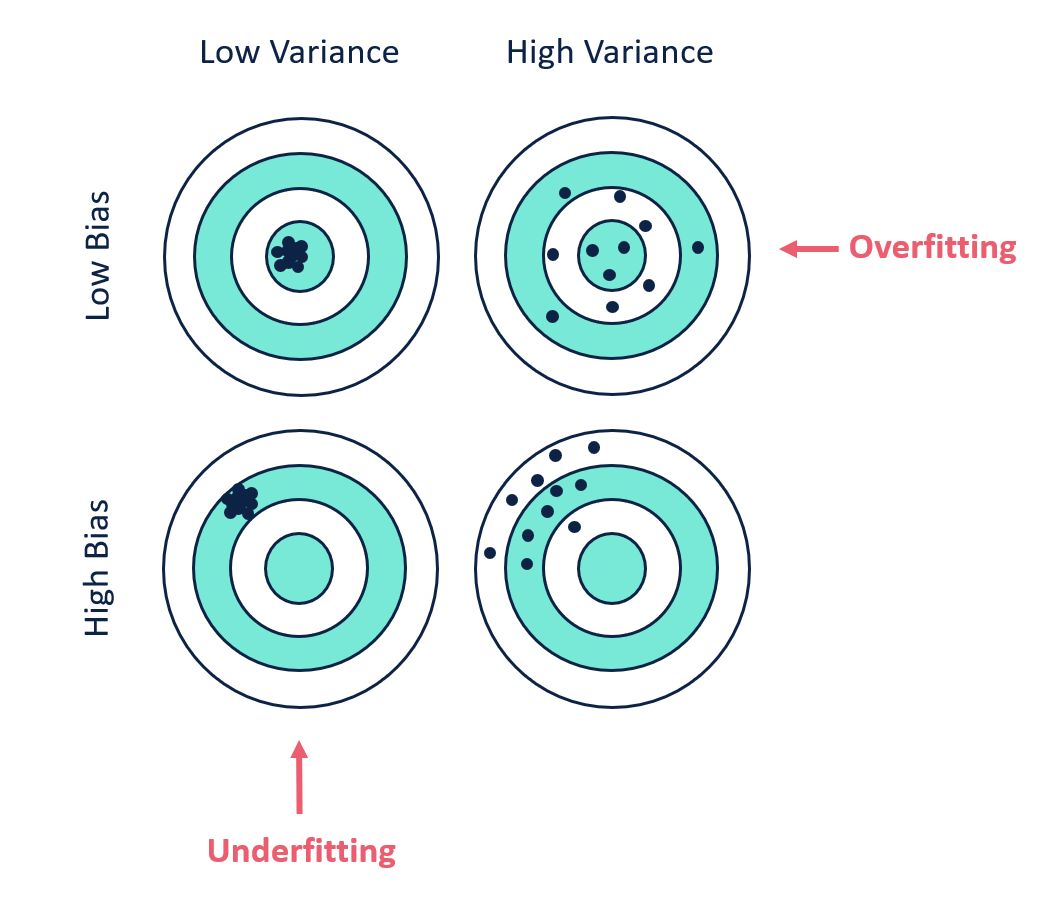
\includegraphics[width=.6\textwidth]{capitulo_marcoteorico/biasVVariance}
    \caption{Sesgo y varianza y su relación con el infra-ajuste y el sobre-ajuste}\label{fig:biasvvariance}
\end{figure}

% \subsubsection{Diagnosticar rendimiento de un modelo}

% Para saber si el modelo esta infra-ajustado o sobre-ajustado, se utiliza la
% curva de aprendizaje, que es 

\subsubsection{Dilema sesgo-varianza}

En la vida real, reducir el sesgo incrementa la varianza y viceversa. Lo óptimo
es encontrar un balance entre los dos para minimizar el error total de
generalización. Desafortunadamente no hay una forma fácil de encontrar este
balance. Es por ello que se requieren múltiples iteraciones de entrenamiento de
uno o varios modelos para encontrar este punto de equilibrio
(\autoref{fig:tradeoff})\cite{F}.

\begin{figure}[H]
    \centering
    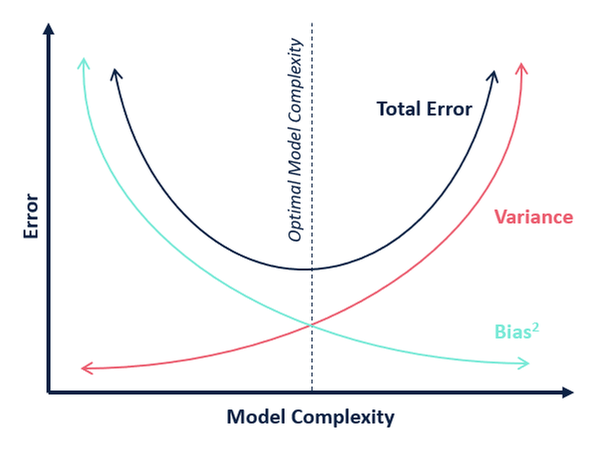
\includegraphics[width=.5\textwidth]{capitulo_marcoteorico/tradeoff}
    \caption{El dilema sesgo-varianza}\label{fig:tradeoff}
\end{figure}

\subsection{Evaluación de un modelo de clasificación}

Se eligió un subconjunto de estas métricas que son comunes en el área de
clasificación médica. Si bien la Exactitud es la métrica más común
aplicada para problemas de clasificación y es la usada como métrica para evaluar
un modelo durante su entrenamiento, no siempre es la mejor opción, ya que asigna
el mismo valor a los Falsos Positivos y a los Falsos Negativos. Para el área
médica, se tiene que tener especial cuidado en medir los errores de
clasificación de un algoritmo puesto que se está tratando de vidas humanas; no
queremos decirle a un paciente que está sano cuando en realidad está enfermo, ni
queremos decirle a un paciente sano que sufre una enfermedad.

Es por ello que tenemos que hacer uso de otras métricas, varias de ellas, para
poder evaluar correctamente el poder de clasificación de un modelo. Tenemos tres
grupos de estas métricas: los valores generales, las métricas usadas para
evaluar y entrenar el modelo y las pruebas de diagnóstico usadas en medicina
basada en evidencias.

Finalmente, se utilizarán Matrices de Confusión que abstraen el rendimiento de
un algoritmo de clasificación. El número de predicciones correctas e incorrectas
es representado por cada clase y muestra todas las formas en las cuales el
modelo de clasificación se confunde entre clases al realizar una predicción.
Estas matrices pueden ser normalizadas con respecto al número total de
predicciones para ofrecer una métrica entre 0 y 1 o sin normalizar para
representar el total de pruebas realizadas.

\subsubsection{Valores generales}

Recordando el conjunto de datos $\mathcal{P}$ usado para probar el modelo,
tenemos dos subconjuntos básicos: el número de positivos ($P$) y el número de
negativos ($N$) que sumados dan la población total ($POP$) de $ \mathbb{D} = P
+ N = POP$. Posteriormente se alimenta el conjunto $\mathcal{P}$ a un algoritmo
de clasificación, se capturan las salidas y se comparan con las etiquetas
verdaderas de cada clase; es decir revisamos si la clase de salida corresponde
con la realidad. De esta acción tomamos cuatro medidas básicas: $TP$, $TN$,
$FP$, $FN$. Los Falsos Positivos corresponden al error estadístico de Tipo I
mientras que los Falsos Negativos corresponden al error de Tipo II
(\autoref{tabla:met_class}).

\begin{table}[H]
    \centering
    \resizebox{\textwidth}{!}{%
    \begin{tabular}{@{}llll@{}}
    \toprule
    Métrica & Nombre & Traducción & Descripción \\ \midrule
    POP & Population & Población & Número de elementos por clase \\
    P & Positive & Positivo & Número de muestras positivas \\
    N & Negative & Negativo & Número de muestras negativas \\
    TP & True Positive & Verdadero Positivo & Detección de la condición cuando si está presente \\
    TN & True Negative & Verdadero Negativo & No detección de la condición cuando no está presente \\
    FP & False Positive & Falso Positivo & Detección de la condición cuando no está presente \\
    FN & False Negative & Falso Negativo & No detección de la condición cuando está presente \\ \bottomrule
    \end{tabular}%
    }
    \caption{Valores generales de un problema de clasificación}\label{tabla:met_class}
    \end{table}

\subsubsection{Métricas evaluadas}

Como mencionamos anteriormente, existen mejores métricas que la Exactitud para
determinar el rendimiento de un algoritmo de clasificación aplicado al área
médica. Posteriormente elegiremos tres para medir el rendimiento del algoritmo
durante el entrenamiento: ACC, TPR (sensibilidad) y TNR (especificidad). 

Otras métricas importantes son el Área bajo la Curva (AUC) que representa que
tan bien nuestro modelo es capaz de distinguir entre clases y que puede ser
graficada. El Índice de Jaccard será usado posteriormente para determinar el
rendimiento en entrenamiento de otro tipo de modelos. Toda esta batería de pruebas
está pensada para estimar lo más correcto posible la capacidad del modelo de clasificar
correctamente entre una célula normal a una anormal y nos da una base sólida para afirmar
el rendimiento real en aplicaciones médicas. La explicación y fórmulas de estás métricas las
podemos encontrar en la \autoref{tabla:breve}. 

% \ecuacionn{ACC = \frac{TP+TN}{P+N} = \frac{TP+TN}{TP+TN+FP+FN}}{Accuracy}
% \ecuacionn{AUC = \frac{TNR+TPR}{2}}{Area under ROC Curve}
% \ecuacionn{BM = TPR + TNR -1}{Bookmaker Informedness}
% \ecuacionn{CEN_{j} = - \sum_{k=1,k\neq j}^{|C|}\left(P_{j,k}^{j}\log_{2(|C|-1)}(P_{j,k}^{j}) + P_{k,j}^{j}\log_{2(|C|-1)}(P_{k,j}^{j})\right)}{Confusion Entropy}
% \ecuacionn{ERR = \frac{FP+FN}{P+N}=\frac{FP+FN}{TP+TN+FP+FN}=1-ACC}{Error Rate}
% \ecuacionn{F1 =  2\frac{PPV \cdot TPR}{PPV + TPR}}{F1 Score}
% \ecuacionn{FDR = \frac{FP}{FP + TP = 1 - PPV}}{False Discovery Rate}
% \ecuacionn{FNR = \frac{FN}{P} = \frac{FN}{FN+TP} = 1 - TPR}{False Negative Rate}
% \ecuacionn{FOR = \frac{FN}{FN+TN} = 1 - NPV}{False Omission Rate}
% \ecuacionn{FPR = \frac{FP}{N} = \frac{FP}{FP+TN}=1-TNR}{False Positive Rate}
% \ecuacionn{J(y, \hat{y}) = \frac{|y\cap\hat{y}|}{|y\cup\hat{y}|} = \frac{|y\cap\hat{y}|}{|y| + |\hat{y} - |y\cap\hat{y}|}}{Jaccard Index}
% \ecuacionn{MCEN_{j} = - \sum_{k=1,k\neq j}^{|C|}\left(P_{j,k}^{j}\log_{2(|C|-1)}(P_{j,k}^{j}) + P_{k,j}^{j}\log_{2(|C|-1)}(P_{k,j}^{j}) \right)}{Modified Confusion Entropy}
% \ecuacionn{NPV = \frac{TN}{TN+FN}}{Negative Predictive Value}
% \ecuacionn{PPV = \frac{TP}{TP+FP}}{Positive Predictive Value}
% \ecuacionn{PRE = \frac{P}{POP}}{Prevalence}
% \ecuacionn{TNR = \frac{TN}{N}=\frac{TN}{TN+FP}}{True Negative Rate}
% \ecuacionn{TPR = \frac{TP}{P} = frac{TP}{TP+FN}}{True Positive Rate}

% \ecuacionn{}{}

\linespread{0.5}
\begin{table}[H]
    \centering
    \resizebox{\textwidth}{!}{%
    \begin{tabular}{@{}p{2cm}p{2cm}p{2cm}p{5cm}p{10cm}@{}}
    \toprule
    Métrica & Nombre & Traducción & Descripción & Fórmula \\ \midrule
    ACC & Accuracy & Exactitud & Número de predicciones correctas de todas las predicciones & \ecuacionn{ACC = \frac{TP+TN}{P+N} = \frac{TP+TN}{TP+TN+FP+FN}}{Accuracy} \\
    AUC & Area under ROC curve & Área bajo la curva ROC & Corresponde a la media aritmética de la sensibilidad y especificidad para cada clase & \ecuacionn{AUC = \frac{TNR+TPR}{2}}{Area under ROC Curve} \\
    BM & Bookmaker Informedness & Información de Bookmaker & Probabilidad de que el algoritmo tome una decisión correcta en oposición a simple adivinanza & \ecuacionn{BM = TPR + TNR -1}{Bookmaker Informedness} \\
    CEN & Confusion Entropy & Entropía de Confusión & Evalúa la confusión a nivel clase basada en la entropía de las matrices de confusión, estadísticamente es más discriminante que ACC & \ecuacionn{CEN_{j} = - \sum_{k=1,k\neq j}^{|C|}\left(P_{j,k}^{j}\log_{2(|C|-1)}(P_{j,k}^{j}) + P_{k,j}^{j}\log_{2(|C|-1)}(P_{k,j}^{j})\right)}{Confusion Entropy} \\
    ERR & Error Rate & Tasa de Error & Número de predicciones incorrectas de todas las predicciones & \ecuacionn{ERR = \frac{FP+FN}{P+N}=\frac{FP+FN}{TP+TN+FP+FN}=1-ACC}{Error Rate} \\
    F1 & F1 Score & Medida F1 & Es el promedio armónico de la precisión y recall, cuyo peor valor es 0 y el mejor 1 & \ecuacionn{F1 =  2\frac{PPV \cdot TPR}{PPV + TPR}}{F1 Score} \\
    FDR & False Discovery Rate & Tasa de Falso Descubrimiento & Permite analizar la proporción de hipótesis nulas rechazadas que son falsas (rechazos incorrectos) & \ecuacionn{FDR = \frac{FP}{FP + TP = 1 - PPV}}{False Discovery Rate} \\
    FNR & False Negative Rate & Tasa de Falsos Negativos & Proporción de positivos que dieron negativos en la prueba & \ecuacionn{FNR = \frac{FN}{P} = \frac{FN}{FN+TP} = 1 - TPR}{False Negative Rate} \\
    FOR & False Omission Rate & Tasa de Falsa Omisión & Mide la proporción de falsos negativos que son incorrectamente rechazados & \ecuacionn{FOR = \frac{FN}{FN+TN} = 1 - NPV}{False Omission Rate} \\
    FPR & False Positive Rate & Tasa de Falsos Positivos & Proporción de todos los negativos que aún así salieron positivos, es equivalente al nivel de significancia. La Especificidad de una prueba es 1 - FPR & \ecuacionn{FPR = \frac{FP}{N} = \frac{FP}{FP+TN}=1-TNR}{False Positive Rate} \\
    J & Jaccard Index & Índice de Jaccard & También conocido como Intersección Sobre Unión (IOU), mide la similitud y diversidad de los conjuntos de muestra & \ecuacionn{J(y, \hat{y}) = \frac{|y\cap\hat{y}|}{|y\cup\hat{y}|} = \frac{|y\cap\hat{y}|}{|y| + |\hat{y} - |y\cap\hat{y}|}}{Jaccard Index} \\
    MCEN & Modified Confusion Entropy & Entropía de Confusión Modificada & Es más robusta estadísticamente que su versión anterior & \ecuacionn{MCEN_{j} = - \sum_{k=1,k\neq j}^{|C|}\left(P_{j,k}^{j}\log_{2(|C|-1)}(P_{j,k}^{j}) + P_{k,j}^{j}\log_{2(|C|-1)}(P_{k,j}^{j}) \right)}{Modified Confusion Entropy} \\
    NPV & Negative Predictive Value & Valor Predictivo Negativo & Proporción de negativos que corresponden a ausencia de condición & \ecuacionn{NPV = \frac{TN}{TN+FN}}{Negative Predictive Value} \\
    PPV & Positive Predictive Value & Valor Predictivo Positivo & Precisión, proporción de positivos que corresponden a la presencia de condición & \ecuacionn{PPV = \frac{TP}{TP+FP}}{Positive Predictive Value} \\
    PRE & Prevalence & Prevalencia & Número de casos de una enfermedad que están presente en una población & \ecuacionn{PRE = \frac{P}{POP}}{Prevalence} \\
    TNR & True Negative Rate & Tasa de Verdaderos Negativos & Especificidad, mide la proporción de negativos que son correctamente clasificados & \ecuacionn{TNR = \frac{TN}{N}=\frac{TN}{TN+FP}}{True Negative Rate} \\
    TPR & True Positive Rate & Tasa de Falsos Positivos & Sensibilidad o recall, mide la proporción de positivos que son identificados como tales & \ecuacionn{TPR = \frac{TP}{P} = frac{TP}{TP+FN}}{True Positive Rate} \\ \bottomrule
    \end{tabular}%
    }
    \caption{Breve explicación de las métricas}\label{tabla:breve}
    \end{table}



% \linespread{0.5}
% \begin{table}[H]
%     \centering
%     \resizebox{\textwidth}{!}{%
%     \begin{tabular}{@{}p{2cm}p{2cm}p{2cm}p{5cm}p{10cm}@{}}
%     \toprule
%     Métrica & Nombre & Traducción & Descripción & Fórmula \\ \midrule
%     ACC & Accuracy & Exactitud & Número de predicciones correctas de todas las predicciones & \ecuacionn{ACC = \frac{TP+TN}{P+N} = \frac{TP+TN}{TP+TN+FP+FN}}{Accuracy} \\
%     AUC & Area under ROC curve & Área bajo la curva ROC & Corresponde a la media aritmética de la sensibilidad y especificidad para cada clase & \(AUC = \frac{TNR+TPR}{2} \) \\
%     BM & Bookmaker Informedness & Información de Bookmaker & Probabilidad de que el algoritmo tome una decisión correcta en oposición a simple adivinanza & \(BM = TPR + TNR -1 \) \\
%     CEN & Confusion Entropy & Entropía de Confusión & Evalúa la confusión a nivel clase basada en la entropía de las matrices de confusión, estadísticamente es más discriminante que ACC & \(CEN_{j} = - \sum_{k=1,k\neq j}^{|C|}\left(P_{j,k}^{j}\log_{2(|C|-1)}(P_{j,k}^{j}) + P_{k,j}^{j}\log_{2(|C|-1)}(P_{k,j}^{j})\right)\) \\
%     ERR & Error Rate & Tasa de Error & Número de predicciones incorrectas de todas las predicciones & \(ERR = \frac{FP+FN}{P+N}=\frac{FP+FN}{TP+TN+FP+FN}=1-ACC \) \\
%     F1 & F1 Score & Medida F1 & Es el promedio armónico de la precisión y recall, cuyo peor valor es 0 y el mejor 1 & \( F1 =  2\frac{PPV \cdot TPR}{PPV + TPR}\) \\
%     FDR & False Discovery Rate & Tasa de Falso Descubrimiento & Permite analizar la proporción de hipótesis nulas rechazadas que son falsas (rechazos incorrectos) & \(FDR = \frac{FP}{FP + TP = 1 - PPV}\) \\
%     FNR & False Negative Rate & Tasa de Falsos Negativos & Proporción de positivos que dieron negativos en la prueba & \( FNR = \frac{FN}{P} = \frac{FN}{FN+TP} = 1 - TPR\) \\
%     FOR & False Omission Rate & Tasa de Falsa Omisión & Mide la proporción de falsos negativos que son incorrectamente rechazados & \(FOR = \frac{FN}{FN+TN} = 1 - NPV \) \\
%     FPR & False Positive Rate & Tasa de Falsos Positivos & Proporción de todos los negativos que aún así salieron positivos, es equivalente al nivel de significancia. La Especificidad de una prueba es 1 - FPR & \(FPR = \frac{FP}{N} = \frac{FP}{FP+TN}=1-TNR \) \\
%     J & Jaccard Index & Índice de Jaccard & También conocido como Intersección Sobre Unión (IOU), mide la similitud y diversidad de los conjuntos de muestra & \( J(y, \hat{y}) = \frac{|y\cap\hat{y}|}{|y\cup\hat{y}|} = \frac{|y\cap\hat{y}|}{|y| + |\hat{y} - |y\cap\hat{y}|}\) \\
%     MCEN & Modified Confusion Entropy & Entropía de Confusión Modificada & Es más robusta estadísticamente que su versión anterior & \(MCEN_{j} = - \sum_{k=1,k\neq j}^{|C|}\left(P_{j,k}^{j}\log_{2(|C|-1)}(P_{j,k}^{j}) + P_{k,j}^{j}\log_{2(|C|-1)}(P_{k,j}^{j}) \right) \) \\
%     NPV & Negative Predictive Value & Valor Predictivo Negativo & Proporción de negativos que corresponden a ausencia de condición & \(NPV = \frac{TN}{TN+FN} \) \\
%     PPV & Positive Predictive Value & Valor Predictivo Positivo & Precisión, proporción de positivos que corresponden a la presencia de condición & \(PPV = \frac{TP}{TP+FP} \) \\
%     PRE & Prevalence & Prevalencia & Número de casos de una enfermedad que están presente en una población & \( PRE = \frac{P}{POP}\) \\
%     TNR & True Negative Rate & Tasa de Verdaderos Negativos & Especificidad, mide la proporción de negativos que son correctamente clasificados & \( TNR = \frac{TN}{N}=\frac{TN}{TN+FP}\) \\
%     TPR & True Positive Rate & Tasa de Falsos Positivos & Sensibilidad o recall, mide la proporción de positivos que son identificados como tales & \( TPR = \frac{TP}{P} = frac{TP}{TP+FN}\) \\ \bottomrule
%     \end{tabular}%
%     }
%     \caption{Breve explicación de las métricas}\label{tabla:breve}
%     \end{table}

\subsubsection{Pruebas de diagnóstico}

Las métricas de prueba de diagnóstico surgen de la necesidad de estimar
correctamente una prueba de diagnóstico médico y fueron pensadas para tomar decisiones en la
medicina basada en evidencias. Sirven para evaluar que tan buena es una prueba de diagnóstico
y tienen ventajas sobre TNR y TPR ya que son menos propensas a cambiar dada la prevalencia de
la enfermedad en el conjunto de evaluación (\autoref{tabla:breve_diag}). 

% \ecuacionn{LR_{+} = PLR = \frac{TPR}{FPR}}{Positive Likelihood Ratio}
% \ecuacionn{LR_{-} = NLR = \frac{FNR}{TNR}}{Negative Likelihood Ratio}
% \ecuacionn{DOR = \frac{LR_{+}}{LR_{-}}}{Diagnostic Odds Ratio}
% \ecuacionn{DP = \frac{\sqrt{3}}{pi}\left((\log_{10}\frac{TPR}{1-TPR}) + (\log_{10}\frac{TNR}{1-TNR})\right)}{Discriminant Power}
% \ecuacionn{IS = -\log_{2}(\frac{TP+FN}{POP}) + \log_{2}(\frac{TP}{TP+FP})}{Information Score}

\linespread{0.5}
\begin{table}[H]
    \centering
    \resizebox{\textwidth}{!}{%
    \begin{tabular}{@{}p{2cm}p{2cm}p{2cm}p{5cm}p{10cm}@{}}
    \toprule
    Métrica & Nombre & Traducción & Descripción & Fórmula \\ \midrule
    PLR & Positive Likelihood Ratio & Razón de Verosimilitud Positiva & Usa la sensibilidad y la especificidad para determinar si el resultado de la prueba cambia la probabilidad de que una condición exista & \ecuacionn{LR_{+} = PLR = \frac{TPR}{FPR}}{Positive Likelihood Ratio} \\
    NLR & Negative Likelihood Ratio & Razón de Verosimilitud Negativa & La probabilidad de que una muestra que dio negativo en la prueba dividido por la probabilidad de que esa muestra sea negativa & \ecuacionn{LR_{-} = NLR = \frac{FNR}{TNR}}{Negative Likelihood Ratio} \\
    DOR & Diagnostic Odds Ratio & Razón de Oportunidades de Diagnóstico & Es la medida de la efectividad de una prueba de diagnóstico, es la proporción de las probabilidades de una prueba de ser positiva si la muestra tiene la enfermedad relativa a las probabilidades de que la prueba sea positiva si el sujeto no tiene la enfermedad &\ecuacionn{DOR = \frac{LR_{+}}{LR_{-}}}{Diagnostic Odds Ratio} \\
    DP & Discriminant Power & Poder Discriminador & Una medida que encapsula la sensibilidad y la especificidad & \ecuacionn{DP = \frac{\sqrt{3}}{pi}\left((\log_{10}\frac{TPR}{1-TPR}) + (\log_{10}\frac{TNR}{1-TNR})\right)}{Discriminant Power} \\
    IS & Information Score & Medida de Información & Cantidad de información necesaria para clasificar correctamente un ejemplo en una clase determinada & \ecuacionn{IS = -\log_{2}(\frac{TP+FN}{POP}) + \log_{2}(\frac{TP}{TP+FP})}{Information Score} \\ \bottomrule
    \end{tabular}%
    }
    \caption{Breve explicación de las pruebas de diagnóstico}\label{tabla:breve_diag}
    \end{table}
\subsection{Deep Learning}

El Aprendizaje Profundo o \hyperlink{abbr}{DL}, es la más reciente rama de la
\hyperlink{abbr}{IA} y es la que mejores resultados ha tenido de todo el
conjunto de algoritmos que componen esta área multidisciplinaria de
conocimiento. Ha sido implementada exitosamente en la mayoría de las
aplicaciones tecnológicas modernas desde las redes sociales (Facebook,
Instagram), servicios en la nube (Watson, Google) y tiene un futuro prometedor
en todo lo relacionado con la explosión tecnológica del siglo XXI.

El \hyperlink{abbr}{DL}, es capaz de aprender de dentro de los datos, patrones
de información y representaciones profundas de los objetos que analicen. Esta
diferenciación con respecto a las aplicaciones tradicionales de las RNA se logra
mediante arquitecturas profundas, mejoras en técnicas matemáticas, incremento en
tecnología computacional que permiten a la computadora, por si sola, extraer las
características principales de las imágenes y, capa por capa, conocer todos los
patrones intrincados que se codifican en la base de datos de entrenamiento. Esta
capacidad de aprender sucesivamente patrones cada vez más abstractos en cada
capa secuencial, se le conoce como Aprendizaje Jerárquico. 

El \hyperlink{abbr}{DL} ofreció mejor rendimiento en muchas tareas distintas, por ejemplo:

\begin{itemize}
    \item Clasificación de imágenes a niveles casi humanos
    \item Reconocimiento de voz a niveles casi humanos
    \item Transcripción de letra escrita a niveles casi humanos
    \item Ha mejorado la traducción asistida por máquinas
    \item Mejora en la conversión texto-habla
    \item Conducción de autos autónomos
    \item Mejora de búsquedas en la web
    \item Habilidad para contestar preguntas en lenguaje natural
\end{itemize}

En el 2011, los mejores resultados en el reto de \emph{ImageNet} (clasificar
miles de imágenes en cientos de clases), la exactitud rondaba solo el 74.3\%. En
2012 un equipo logró mejorar esta exactitud a 83.6\%. Para el 2015, el ganador
manejaba una precisión del 96.4\% utilizando ConvNets, en la actualidad
\emph{ImageNet} se considera un problema resuelto.

Las dos ideas claves para el \hyperlink{abbr}{DL} aplicado a
\hyperlink{abbr}{VC} fueron las \hyperlink{abbr}{ConvNet}s y el \emph{Algoritmo
de Retro-propagación} (Backpropagation) ya existían hace 30 años. Debido a que
el campo es experimental y no teórico, los avances en algoritmos son posibles
solo cuando hay suficientes datos y Hardware. Estas ideas estuvieron en letargo,
esperando avances en Hardware para ser posibles técnicamente y en la maduración
del concepto de almacenamiento y recopilación de datos \cite{Chollet2018}.

\subsubsection{Hardware}

En 30 años los procesadores disponibles para el usuario final se han vuelto cada
vez más rápidos en un factor de 5000. Ahora es posible entrenar modelos de
\hyperlink{abbr}{DL} en una computadora cualquiera e implementar
\hyperlink{abbr}{DL} dentro de dispositivos con restricciones de rendimiento
como los \hyperlink{abbr}{SE}.

Durante los últimos 20 años, dos compañías se enfrascaron en una batalla
tecnológica para desarrollar veloces unidades de procesamiento en paralelo para
aplicarlas al área de Gráficas Computacionales aplicadas a cuestiones mundanas
como los videojuegos. Una imagen (o video), como vimos anteriormente, se puede
representar como una matriz y es posible aplicarle operaciones de álgebra
lineal. Es por ello que un procesador capaz de paralelizar miles de operaciones
sencillas es el indicado para procesar gráficas pero también imágenes. A este
tipo de procesadores se les llamó Graphical Processing Unit
(\hyperlink{abbr}{GPU}\nomenclature{GPU}{Graphical Processing Unit}), que
básicamente son mini supercomputadora capaz de procesar cientos de matrices y
operaciones en tiempo real, operaciones comunes en el área de gráficos por
computadora y videojuegos. 

Dos empresas se enfrascaron en una batalla tecnológica para capitalizar el
mercado de los videojuegos y catapultaron el desarrollo de estos
\hyperlink{abbr}{GPU}s: Nvidia y AMD. Siendo la primera la ganadora indiscutible
en lo que rendimiento para entrenar algoritmos de \hyperlink{abbr}{DL}, debido a
que es la única que tiene en sus líneas de productos tarjetas específicas para
\hyperlink{abbr}{IA}(\autoref{fig:companias}).


\begin{figure}[H]
    \centering
    \begin{subfigure}{.5\textwidth}
      \centering
      
\includegraphics[width=.5\linewidth]{capitulo_marcoteorico/nvidia-ds.png}
      \caption{Nvidia}
      \label{fig:Nvidia}
    \end{subfigure}%
    \begin{subfigure}{.5\textwidth}
      \centering
      
\includegraphics[width=.5\linewidth]{capitulo_marcoteorico/amd-ds.png}
      \caption{AMD}
      \label{fig:AMD}
    \end{subfigure}
    \caption{Compañías líderes en GPUs}
    \label{fig:companias}
    \end{figure}

Las \hyperlink{abbr}{ConvNet}s consisten, principalmente, en miles de pequeñas
multiplicaciones matriciales, por lo tanto son altamente generalizables. En 2007
Nvidia lanzó Compute Unified Device Architecture
(\hyperlink{abbr}{CUDA}\nomenclature{CUDA}{Compute Unified Device
Architecture}), que permitió programar las \hyperlink{abbr}{GPU}s para ser
aplicadas a la parte científica. En la \autoref{fig:cpuvsgpu} se tiene una
comparativa entre el rendimiento en GFLOPS \cite{Nvidia} \cite{Nvidiaa}. Se nota
claramente la brecha entre el rendimiento de los procesadores centrales
tradicionales y los \hyperlink{abbr}{GPU}s.

\begin{figure}[H]
    \centering
    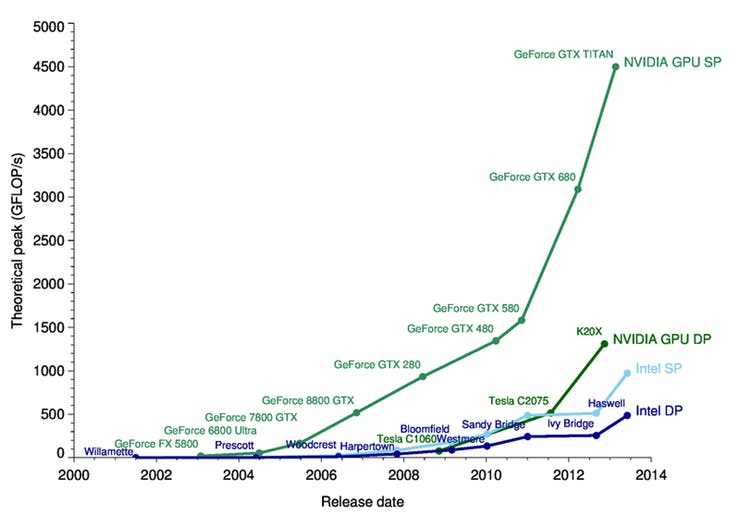
\includegraphics[width=0.7\textwidth]{capitulo_marcoteorico/cpuvsgpu}
    \caption{CPU vs GPU}\label{fig:cpuvsgpu}
\end{figure}

En la actualidad Nvidia cuenta con \hyperlink{abbr}{GPU}s capaces de realizar
más de 14.90 TFLOPS, lo que es equivalente a 14.90 trillones de operaciones de
punto flotante por segundo a una precisión de 32 bits. Permitiendo entrenar en
un día modelos que habrían ganado fácilmente la competencia de \emph{ImageNet}.

La empresa Nvidia tiene un compromiso muy grande por la investigación y es uno
de los actores principales en la revolución del \hyperlink{abbr}{DL}. Es por
ello que han implementado un programa de donación de \hyperlink{abbr}{GPU}s de
muy alto rendimiento para proyectos que cumplan una estricta lista de
requerimientos. El modelo de GPU donado es \emph{Titan V} (\autoref{fig:titan}),
con un costo de \$75,038.34 pesos mexicanos y que cuenta con las siguientes
características.

\begin{itemize}
    \item{\textbf{Arquitectura:}} Volta
    \item{\textbf{Tipo de proceso:}} 12 nanómetros
    \item{\textbf{Transistores:}} 21,100 millones
    \item{\textbf{Interface:}} PCIe 3.0 $\times$ 16
    \item{\textbf{Velocidad:}} 1200Mhz - 1455Mhz
    \item{\textbf{Memoria:}} 12 GB
    \item{\textbf{Ancho de banda:}} 651.3 GB/s 
    \item{\textbf{Núcleos tensoriales:}} 640
    \item{\textbf{Núcleos CUDA:}} 5120
    \item{\textbf{Rendimiento tensorial:}} 110 TFLOPS (11 trillones de operaciones por segundo)
    \item{\textbf{Consumo de poder:}} 200W
\end{itemize}

\begin{figure}[H]
    \centering
    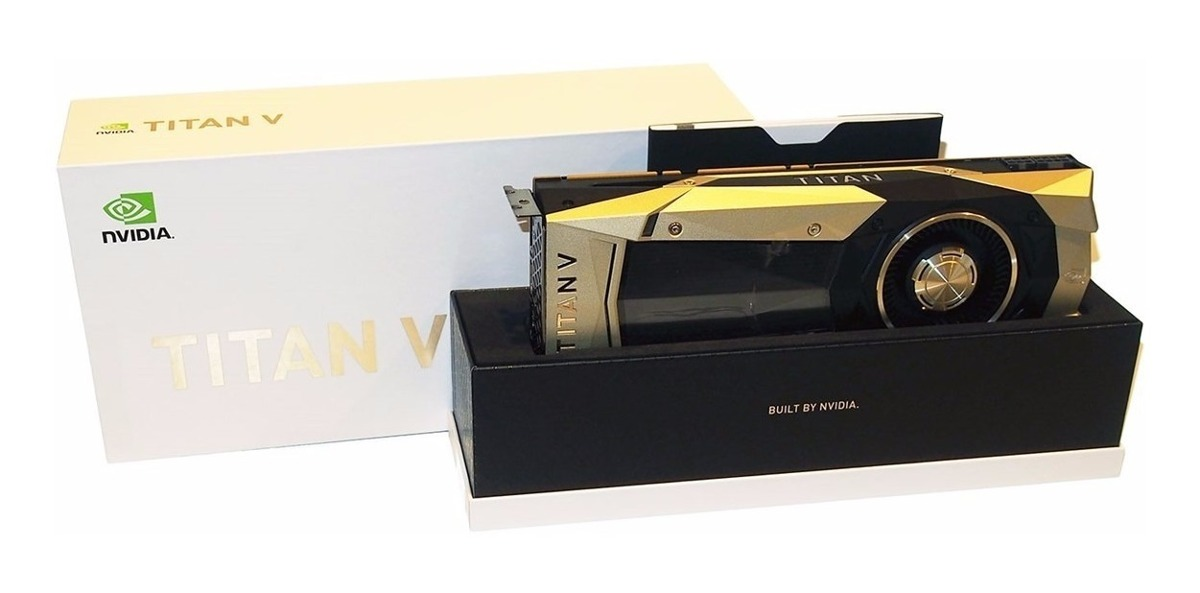
\includegraphics[width=0.7\textwidth]{capitulo_marcoteorico/titan.jpg}
    \caption{Titan V}\label{fig:titan}
\end{figure}

Debido a los objetivos de esta tesis, se tuvo la fortuna de recibir una donación
de una de estas tarjetas gráficas, lo cual catalizó el proceso de desarrollo y
permitió explorar muchas arquitecturas y paradigmas. La propuesta que se mandó a
Nvidia sobre la cual se tomó la decisión para la donación de la tarjeta se puede
encontrar en el \autoref{appendix:grant}.

\subsubsection{Datos}

El darle la importancia necesaria los datos creo las condiciones necesarias para
entrar a la llamada Cuarta Revolución Industrial. El internet permite transmitir
datos fácilmente a través de continentes y también permite colectar y distribuir
BDs libres para desarrollar y probar nuevos algoritmos de \hyperlink{abbr}{IA}. 

Uno de las \hyperlink{abbr}{BD}s más famosas es la de \emph{ImageNet}
(\autoref{fig:imagenet}) que consiste en 1.4 millones de imágenes para ser
categorizadas en 1000 clases distintas; se subdivide en 1.3 millones de imágenes
para entrenamiento, 50000 para validación y 100000 de prueba. Es esta
\hyperlink{abbr}{BD} la que posteriormente se reentrenará y ajustará para
clasificar imágenes en clases que nunca antes ha visto. Esto es lo que se conoce
como \hyperlink{abbr}{TL}. Al final dos bases de datos trabajarán en conjunto
para generar clasificadores específicos. Reduciendo mucho el tiempo de
desarrollo, el tiempo de entrenamiento y la cantidad de datos necesaria para
alcanzar un buen rendimiento \cite{Russakovsky2015}.

\begin{figure}[H]
    \centering
    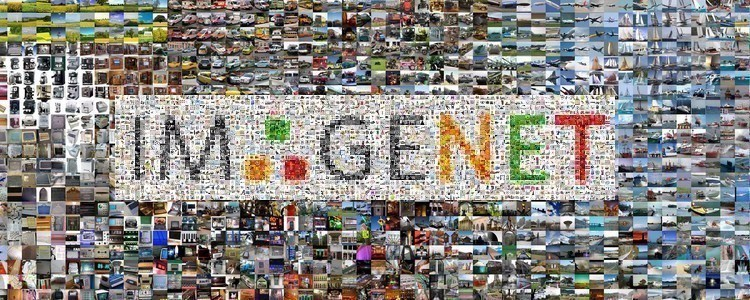
\includegraphics[width=0.7\textwidth]{capitulo_marcoteorico/imagenet}
    \caption{ImageNet}\label{fig:imagenet}
\end{figure}


\subsubsection{Redes neuronales convolucionales}

Las \hyperlink{abbr}{ConvNet}s son probablemente la epítome y el más grande éxito
en la historia de los algoritmos inspirados por la naturaleza. Las claves de su
diseño fueron inspiradas por las neurociencias.

Todo comienza con los estudios neurocientíficos realizados por David Hubel y
Torsten Wiesel para descubrir como es que funciona en su forma más básica el
sistema de visión de los mamíferos. Finalmente ganaron el premio Nobel. Se
observó como el cerebro de cierto mamífero responde a las imágenes proyectadas
en una pantalla. El momento Eureka fue cuando se descubrió que las neuronas en
las etapas iniciales del sistema respondían de una forma a ciertos patrones de
luz, como aquellos semejantes a barras pero que no lo se activaban con otros
patrones \cite{Learningb}.

Las \hyperlink{abbr}{RNA} comunes que usan la multiplicación matricial para
operar de la entrada a la salida, lo que significa que cada salida interactúa
con cada entrada. Las \hyperlink{abbr}{ConvNet}s no hacen esto, ya que tienen
conexiones dispersas lo que nos permite operar con menos parámetros lo que
reduce la memoria requerida por el modelo y también incrementa la eficiencia
estadística al ser un modelo menos complejo.

Entrenar una red es un proceso donde se toma una imagen, se pasa por las
\textbf{capas} de la red, se toma la salida y se compara con la etiqueta real
con una \textbf{función de pérdida}, que es lo que tomará el
\textbf{optimizador} para actualizar los pesos de las capas y así generar
aprendizaje (\autoref{fig:convnetfuncionamiento}). Son estos últimos dos pasos
los que constituyen la fase de entrenamiento \cite{Chollet2018}. 

\begin{figure}[H]
    \centering

    \tikzset{every picture/.style={line width=0.75pt}} %set default line width to 0.75pt        

    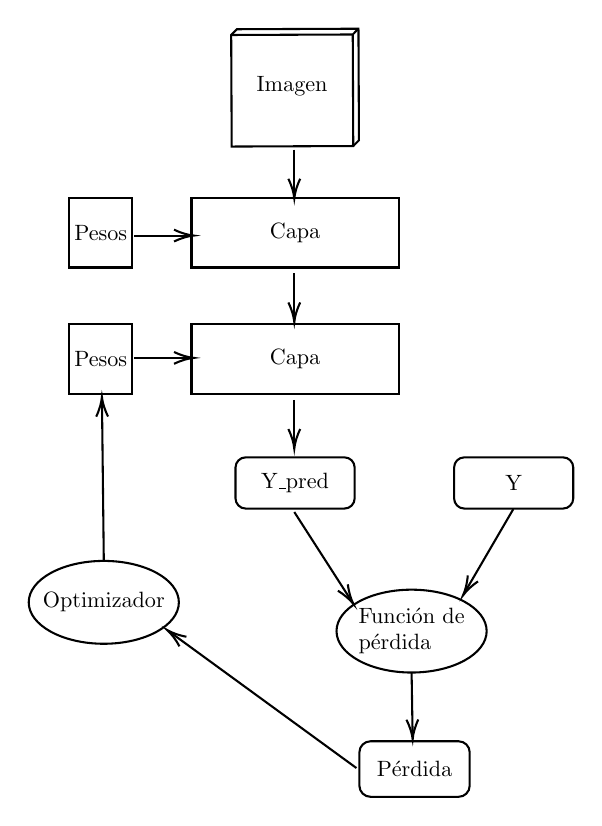
\begin{tikzpicture}[x=0.65pt,y=0.65pt,yscale=-1,xscale=1]
    %uncomment if require: \path (0,466.8999938964844); %set diagram left start at 0, and has height of 466.8999938964844
    
    %Shape: Cube [id:dp572074485163177] 
    \draw   (338.56,11.69) -- (341.73,8.49) -- (409.31,8.2) -- (409.59,70.22) -- (406.42,73.42) -- (338.84,73.71) -- cycle ; \draw   (409.31,8.2) -- (406.14,11.41) -- (338.56,11.69) ; \draw   (406.14,11.41) -- (406.42,73.42) ;
    %Shape: Rectangle [id:dp03598082060301744] 
    \draw   (316.49,102.24) -- (431.66,102.24) -- (431.66,140.94) -- (316.49,140.94) -- cycle ;
    %Rounded Rect [id:dp3134786406771225] 
    \draw   (340.95,252.18) .. controls (340.95,249.04) and (343.5,246.49) .. (346.64,246.49) -- (401.51,246.49) .. controls (404.65,246.49) and (407.2,249.04) .. (407.2,252.18) -- (407.2,269.26) .. controls (407.2,272.41) and (404.65,274.96) .. (401.51,274.96) -- (346.64,274.96) .. controls (343.5,274.96) and (340.95,272.41) .. (340.95,269.26) -- cycle ;
    %Shape: Ellipse [id:dp6480096513963544] 
    \draw   (397.11,343.08) .. controls (397.11,330.36) and (415.8,320.05) .. (438.85,320.05) .. controls (461.9,320.05) and (480.58,330.36) .. (480.58,343.08) .. controls (480.58,355.8) and (461.9,366.11) .. (438.85,366.11) .. controls (415.8,366.11) and (397.11,355.8) .. (397.11,343.08) -- cycle ;
    %Rounded Rect [id:dp24423709699512997] 
    \draw   (409.83,410.51) .. controls (409.83,407.1) and (412.6,404.33) .. (416.01,404.33) -- (464.98,404.33) .. controls (468.38,404.33) and (471.15,407.1) .. (471.15,410.51) -- (471.15,429.03) .. controls (471.15,432.44) and (468.38,435.2) .. (464.98,435.2) -- (416.01,435.2) .. controls (412.6,435.2) and (409.83,432.44) .. (409.83,429.03) -- cycle ;
    %Shape: Rectangle [id:dp43144278502463307] 
    \draw   (316.49,172.6) -- (431.66,172.6) -- (431.66,211.3) -- (316.49,211.3) -- cycle ;
    %Rounded Rect [id:dp5373852672510785] 
    \draw   (462.48,252.18) .. controls (462.48,249.04) and (465.03,246.49) .. (468.18,246.49) -- (523.04,246.49) .. controls (526.18,246.49) and (528.73,249.04) .. (528.73,252.18) -- (528.73,269.26) .. controls (528.73,272.41) and (526.18,274.96) .. (523.04,274.96) -- (468.18,274.96) .. controls (465.03,274.96) and (462.48,272.41) .. (462.48,269.26) -- cycle ;
    %Shape: Ellipse [id:dp07918073027327166] 
    \draw   (226,327.09) .. controls (226,314.37) and (244.69,304.06) .. (267.74,304.06) .. controls (290.79,304.06) and (309.47,314.37) .. (309.47,327.09) .. controls (309.47,339.81) and (290.79,350.12) .. (267.74,350.12) .. controls (244.69,350.12) and (226,339.81) .. (226,327.09) -- cycle ;
    %Shape: Rectangle [id:dp407034174459763] 
    \draw   (248.6,102.24) -- (283.59,102.24) -- (283.59,140.94) -- (248.6,140.94) -- cycle ;
    %Shape: Rectangle [id:dp8903310031572068] 
    \draw   (248.6,172.6) -- (283.59,172.6) -- (283.59,211.3) -- (248.6,211.3) -- cycle ;
    %Straight Lines [id:da9503378258448546] 
    \draw    (373.64,75.37) -- (373.64,100.56) ;
    \draw [shift={(373.64,102.56)}, rotate = 270] [color={rgb, 255:red, 0; green, 0; blue, 0 }  ][line width=0.75]    (10.93,-3.29) .. controls (6.95,-1.4) and (3.31,-0.3) .. (0,0) .. controls (3.31,0.3) and (6.95,1.4) .. (10.93,3.29)   ;
    
    %Straight Lines [id:da6538108644651045] 
    \draw    (373.64,144.14) -- (373.64,169.32) ;
    \draw [shift={(373.64,171.32)}, rotate = 270] [color={rgb, 255:red, 0; green, 0; blue, 0 }  ][line width=0.75]    (10.93,-3.29) .. controls (6.95,-1.4) and (3.31,-0.3) .. (0,0) .. controls (3.31,0.3) and (6.95,1.4) .. (10.93,3.29)   ;
    
    %Straight Lines [id:da11465436892873382] 
    \draw    (373.64,214.5) -- (373.64,239.69) ;
    \draw [shift={(373.64,241.69)}, rotate = 270] [color={rgb, 255:red, 0; green, 0; blue, 0 }  ][line width=0.75]    (10.93,-3.29) .. controls (6.95,-1.4) and (3.31,-0.3) .. (0,0) .. controls (3.31,0.3) and (6.95,1.4) .. (10.93,3.29)   ;
    
    %Straight Lines [id:da8812877925296484] 
    \draw    (373.64,276.87) -- (405.46,326.37) ;
    \draw [shift={(406.54,328.05)}, rotate = 237.26] [color={rgb, 255:red, 0; green, 0; blue, 0 }  ][line width=0.75]    (10.93,-3.29) .. controls (6.95,-1.4) and (3.31,-0.3) .. (0,0) .. controls (3.31,0.3) and (6.95,1.4) .. (10.93,3.29)   ;
    
    %Straight Lines [id:da7901209543223828] 
    \draw    (495.39,275.27) -- (468.43,321.52) ;
    \draw [shift={(467.42,323.25)}, rotate = 300.24] [color={rgb, 255:red, 0; green, 0; blue, 0 }  ][line width=0.75]    (10.93,-3.29) .. controls (6.95,-1.4) and (3.31,-0.3) .. (0,0) .. controls (3.31,0.3) and (6.95,1.4) .. (10.93,3.29)   ;
    
    %Straight Lines [id:da8658316280685309] 
    \draw    (438.85,366.11) -- (439.42,401.22) ;
    \draw [shift={(439.45,403.21)}, rotate = 269.07] [color={rgb, 255:red, 0; green, 0; blue, 0 }  ][line width=0.75]    (10.93,-3.29) .. controls (6.95,-1.4) and (3.31,-0.3) .. (0,0) .. controls (3.31,0.3) and (6.95,1.4) .. (10.93,3.29)   ;
    
    %Straight Lines [id:da7857093875683684] 
    \draw    (408.19,419.21) -- (304.51,343.62) ;
    \draw [shift={(302.89,342.44)}, rotate = 396.09000000000003] [color={rgb, 255:red, 0; green, 0; blue, 0 }  ][line width=0.75]    (10.93,-3.29) .. controls (6.95,-1.4) and (3.31,-0.3) .. (0,0) .. controls (3.31,0.3) and (6.95,1.4) .. (10.93,3.29)   ;
    
    %Straight Lines [id:da501570434777244] 
    \draw    (267.74,304.06) -- (266.72,214.9) ;
    \draw [shift={(266.69,212.9)}, rotate = 449.35] [color={rgb, 255:red, 0; green, 0; blue, 0 }  ][line width=0.75]    (10.93,-3.29) .. controls (6.95,-1.4) and (3.31,-0.3) .. (0,0) .. controls (3.31,0.3) and (6.95,1.4) .. (10.93,3.29)   ;
    
    %Straight Lines [id:da9780612123951469] 
    \draw    (284.73,123.2) -- (315.73,123.2) ;
    \draw [shift={(317.73,123.2)}, rotate = 180] [color={rgb, 255:red, 0; green, 0; blue, 0 }  ][line width=0.75]    (10.93,-3.29) .. controls (6.95,-1.4) and (3.31,-0.3) .. (0,0) .. controls (3.31,0.3) and (6.95,1.4) .. (10.93,3.29)   ;
    
    %Straight Lines [id:da8795550241239272] 
    \draw    (284.73,191.2) -- (315.73,191.2) ;
    \draw [shift={(317.73,191.2)}, rotate = 180] [color={rgb, 255:red, 0; green, 0; blue, 0 }  ][line width=0.75]    (10.93,-3.29) .. controls (6.95,-1.4) and (3.31,-0.3) .. (0,0) .. controls (3.31,0.3) and (6.95,1.4) .. (10.93,3.29)   ;
    
    
    % Text Node
    \draw (372.43,39.87) node [scale=0.8] [align=left] {Imagen};
    % Text Node
    \draw (374.08,121.59) node [scale=0.8] [align=left] {Capa};
    % Text Node
    \draw (374.08,191.95) node [scale=0.8] [align=left] {Capa};
    % Text Node
    \draw (374.08,260.72) node [scale=0.8] [align=left] {Y\_pred};
    % Text Node
    \draw (495.61,260.72) node [scale=0.8] [align=left] {Y};
    % Text Node
    \draw (438.85,343.08) node [scale=0.8] [align=left] {Función de\\pérdida};
    % Text Node
    \draw (440.49,419.77) node [scale=0.8] [align=left] {Pérdida};
    % Text Node
    \draw (267.74,327.09) node [scale=0.8] [align=left] {Optimizador};
    % Text Node
    \draw (266.09,191.95) node [scale=0.8] [align=left] {Pesos};
    % Text Node
    \draw (266.09,121.59) node [scale=0.8] [align=left] {Pesos};
    
    
    \end{tikzpicture}
    
\caption{Diagrama de funcionamiento de una ConvNet}
\label{fig:convnetfuncionamiento}
\end{figure}

\subsubsection{Capas}

Las \hyperlink{abbr}{ConvNet}s están compuestas de las siguientes capas:

\begin{enumerate}
    \item{Capa convolucional}
    \item{Capa de función de activación}
    \item{Pooling}
    \item{Flatten}
    \item{Capa densa}
    \item{Dropout}
    \item{Softmax}
\end{enumerate}

En la \autoref{fig:arch} podemos observar un diagrama de las capas de una
ConvNet. En la cual la primera capa es una imagen de 256 $\times$ 256 $\times$
3. La cual entra al block1 el cual esta compuesto por un tensor de 256 $\times$
256 $\times$ 64, donde el último número representa la cantidad de filtros que se
le van a aplicar a una imagen. El block1 contiene la capa convolucional de
un color naranja claro y la capa de función de activación de un color más opaco.
Posteriormente se procesa la salida en la capa de Pooling la cual la reduce a la
mitad y se alimenta al block2 el cual es un cubo de 128 $\times$ 128 $\times$
128. Luego entra al block3, cuya salida es pasada por la capa Flatten
representada por las líneas punteadas y pasa a la primera capa densa de color
púrpura claro, su respectiva capa de función de activación y la capa de dropout.
Al final ingresa as la capa \emph{Softmax} donde $n$ representa la cantidad de
categorías a clasificar. A este proceso se le conoce como Forward Pass.

\begin{figure}[H]
    \centering
    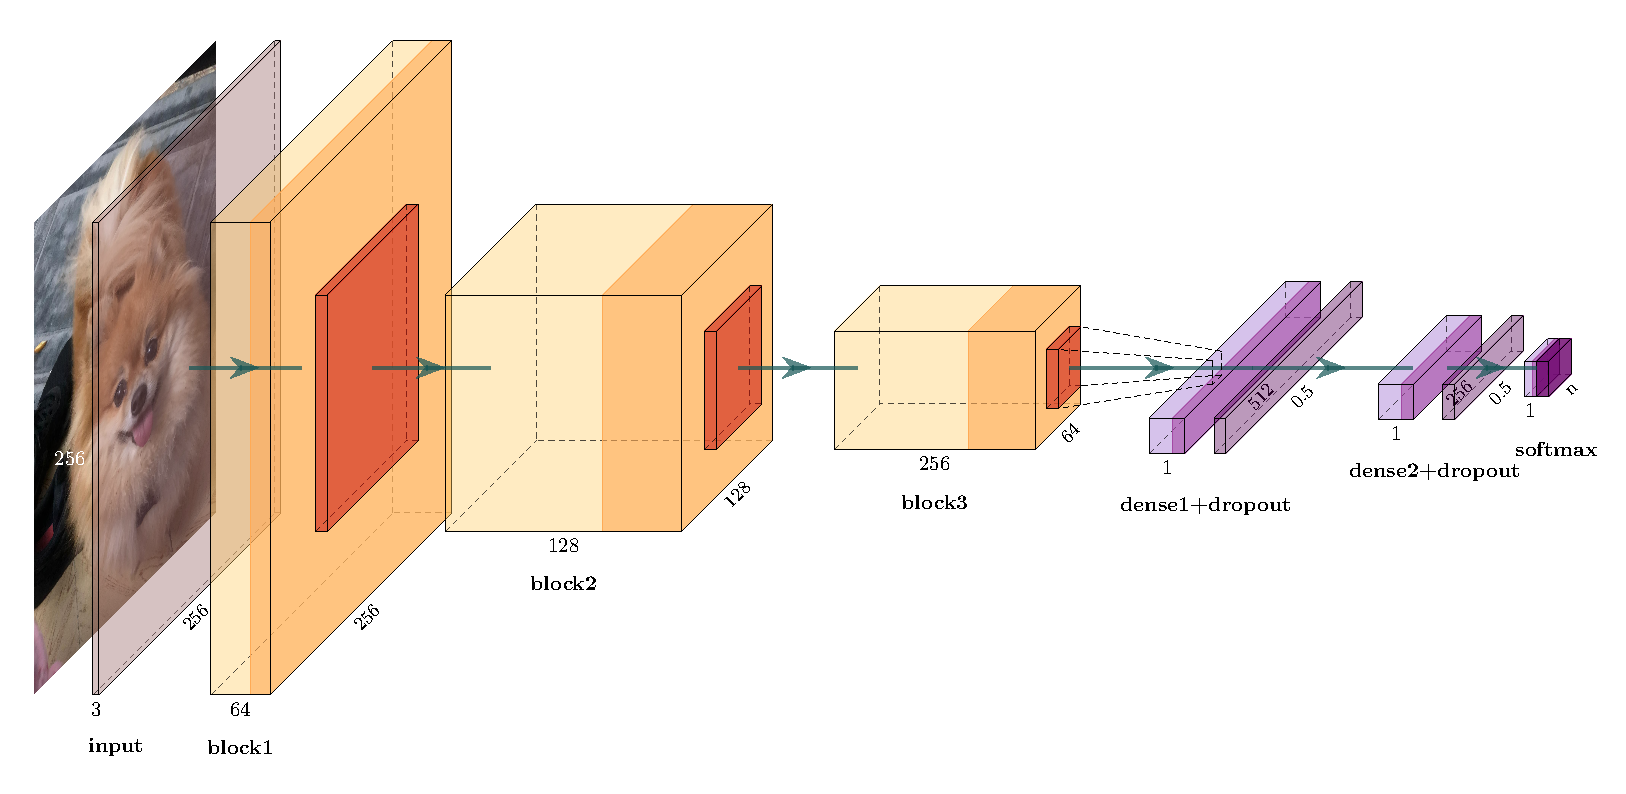
\includegraphics[width=\textwidth]{capitulo_marcoteorico/arch}
    \caption{Diagrama de una ConvNet}\label{fig:arch}
\end{figure}

La \textbf{Capa convolucional} aplica a una imagen a color de 256 $\times$ 256,
es decir, un tensor tridimensional de 256 $\times$ 256 $\times$ 3, una función
matemática llamada convolución (\autoref{Función de convolución}), que es una
operación lineal especializada. Esta operación substituye la tradicional
operación matricial encontrada en las redes neuronales tradicionales. La
convolución capta diferentes medidas dentro de cierto espacio, delimitado por un
filtro (una matriz de grado $n$), la cual aplica una operación que multiplica y
suma la matriz de la imagen de entrada y agrega los datos en un solo punto,
efectivamente codificando un área bidimensional a un solo valor numérico, como
se muestra en la \autoref{fig:conv}:

\ecuacion{h^{(q+1)}_{ijp} = \sum_{r=1}^{F_{q}}\sum_{s=1}^{F_{q}} \sum_{k=1}^{d_{q}} w^{(p,q)}_{rsk} h^{(q)}_{i+r-1, j+s-1,k}}{Función de convolución}

% \begin{equation}
%     \label{eq:conv}
%     h^{(q+1)}_{ijp} = \sum_{r=1}^{F_{q}}\sum_{s=1}^{F_{q}} \sum_{k=1}^{d_{q}} w^{(p,q)}_{rsk} h^{(q)}_{i+r-1, j+s-1,k}
% \end{equation}

\begin{figure}[H]
    \centering
    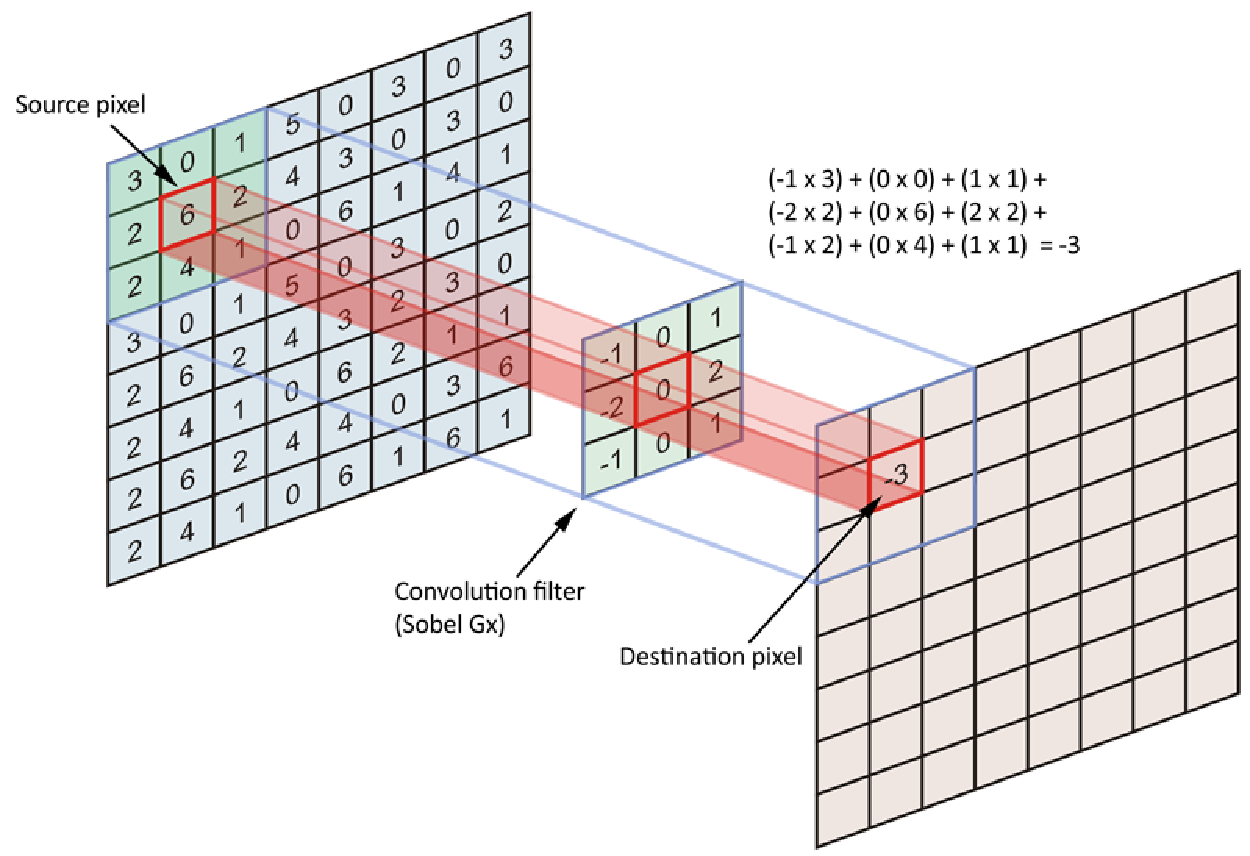
\includegraphics[width=0.6\textwidth]{capitulo_marcoteorico/conv}
    \caption{La convolución aplicada a una imagen}\label{fig:conv}
\end{figure}

La \textbf{Capa de la función de activación} aplica la no linealidad. Existen
muchos tipos de función de activación pero \emph{ReLU} o Rectifier Linear Unit
(\autoref{Rectified Linear Unit}) es la que mejores resultados ha dado en el
área de RNA. Es barata de computar, converge fácil, carece del problema de
desvanecimiento de gradientes (sigmoidal y tanh padecen de esto) y tiene
derivada 0 para todos los negativos y 1 para los positivos.

\ecuacion{  R(z)=\begin{cases}
    0, & \text{if $z<0$}.\\
    1, & \text{otherwise}.
  \end{cases}}{Rectified Linear Unit}

% \begin{equation}
%     \label{eq:relu}
%   R(z)=\begin{cases}
%     0, & \text{if $z<0$}.\\
%     1, & \text{otherwise}.
%   \end{cases}
% \end{equation}

En la \autoref{fig:relu} comparamos las gráficas de sigmoidal y \emph{ReLU}. Se
observa que sigmoidal tiene un rango más amplio de valores y es una fórmula más
compleja. Por el contrario \emph{ReLU} tiene una gráfica bastante sencilla.

\begin{figure}[H]
    \centering
    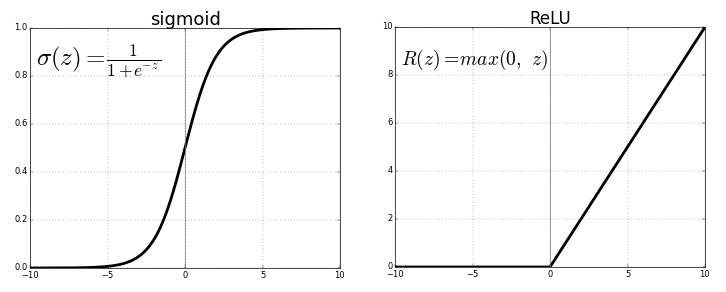
\includegraphics[width=0.7\textwidth]{capitulo_marcoteorico/relu}
    \caption{Comparación entre ReLU y Sigmoidal}\label{fig:relu}
\end{figure}

El \textbf{pooling} (\autoref{fig:pool}) se refiere a una operación que toma
pequeñas regiones de tamaño $P_{q} \times P_{q}$ en cada capa y produce otra de
la misma profundidad. Para cada cuadrado generado por este proceso en cada uno
de los $d_{q}$ filtros, solamente se devuelve el valor máximo. Esto es conocido
como \emph{max pooling} y su fórmula se muestra en la \autoref{MaxPooling2D}.

\ecuacion{h^{n}_{j}(x) = max_{\bar{x} \in N(x), \bar{y} \in N(y)} h^{n-1}_{j} (\bar{x}, \bar{y})}{MaxPooling2D}

\begin{figure}[H]
    \centering
    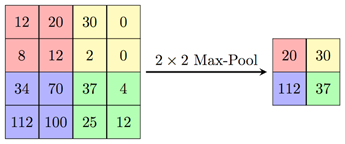
\includegraphics[width=0.4\textwidth]{capitulo_marcoteorico/maxpool}
    \caption{Maxpooling para regiones de $2 \times 2$}\label{fig:pool}
\end{figure}

La capa \textbf{Flatten} convierte el volumen de salida en un vector
unidimensional para poder ser alimentado a la \textbf{capa densa}. La cual no es
más que la clásica capa de RNA del perceptrón multicapa. La cual recibe como
entrada un vector unidimensional y procede a sacar otro vector unidimensional
del tamaño del número de neuronas de la capa. Esta salida puede entrar a la
\textbf{capa dropout} que desactiva secuencialmente neuronas dada cierta
probabilidad lo que efectivamente hace a la red más robusta y reduce el
sobreajuste.

Por último, la \textbf{capa Softmax} (\autoref{Softmax}) es una función de activación que nos
permite realizar clasificación binaria o multi-clase, dependiendo del número de
neuronas que tenga. Colapsa un vector K-dimensional con valores reales y a un
vector K-dimensional cuyos valores se encuentran restringidos a un rango entre 0
y 1 y cuya suma siempre dará 1. Efectivamente convirtiendo cada dimension en una
clase y el valor en una probabilidad de pertenecer o no pertenecer.

\ecuacion{\textsigma(z)_{i} = \frac{e^{z_{i}}}{\sum_{j=1}^{K}}}{Softmax}

\subsubsection{Entrenamiento}

Para alcanzar una precisión aplicable al mundo real, se requiere durante el
entrenamiento una base de datos robusta y que represente fervientemente la
realidad de los datos del problema. Para enriquecer estas bases de datos, se
aplica un pre-proceso sobre las mismas para aumentar la calidad y el tamaño del
conjunto de entrenamiento. Rotando imágenes, generando imágenes espejo,
cambiando contrastes son operaciones básicas a realizar; esto hace que otras
medidas más complejas sean necesarias: poner imágenes en la misma escala,
normalizar mediante medias y desviaciones estándar, aplicación de filtros
gaussianos y afinar proporciones. Esto es conocido como aumentación de datos.

Los hiperparámetros, que son aquellas condiciones de operación del algoritmo que
este no puede aprender por si solo. Son hiperparámetros el Batch Size que rige
la cantidad de imágenes que se necesitan para actualizar los pesos, el algoritmo
de optimización que buscará minimizar la pérdida, la Learning Rate o Tasa de
Aprendizaje del algoritmo de optimización (muy grande y rebotará fuera del
mínimo, muy pequeña y nunca llegará). También lo son el número de capas y la
probabilidad del Dropout \cite{Goodfellow2016}.

Como algoritmo de optimización se usará una variante del clásico Gradiente
Descendente llamada Adaptive Moment Estimation o Adam. El cual presenta ciertas
ventajas con respecto al algoritmo de gradiente (\autoref{fig:adam})
\cite{Kingma2014}:

\begin{itemize}
    \item Fácil de implementar
    \item Computacionalmente eficiente
    \item Pocos requerimientos de memoria
    \item Apropiado para objetos no estacionarios
    \item Sus hiperparámetros internos requieren casi ningún ajuste
\end{itemize}

Adam combina las mejores características de otros algoritmos de optimización
ajustando la tasa de aprendizaje por parámetro aprendido. Teniendo un mejor
rendimiento que las alternativas (\autoref{alg:adam}).

\begin{algorithm}[H]
    \SetAlgoLined
    \SetKwInOut{Input}{Input}\SetKwInOut{Output}{Output}
    \Input{$\alpha: $ Stepsize}
    \Input{$\beta_{1}, \beta_{2} \in [0,1): $ Exponential decay rate}
    \Input{$f(\theta): $ Stochastic objective function}
    \Input{$\theta_{0}: $ Initial parameter vector}
    \Output{$\theta_{t}$}
    \Begin{$m_{0} \longleftarrow 0$ (Initialize first momment vector)
    \BlankLine
    $v_{0}\longleftarrow 0$ (Initialize second momment vector)
    \BlankLine
    $t \longleftarrow 0$ (Initialize timestep)
    \BlankLine
    
    \While{$\theta_{t}$ not converged}{
        $t \longleftarrow t + 1$
        \BlankLine
        $g_{t} \longleftarrow \nabla_{\theta}f_{t}(\theta_{t-1})$ Get gradients w.r.t. stochastic objective at timestep $t$
        \BlankLine
        $m_{t} \longleftarrow \beta_{1} \cdot m_{t-1} + (1 - \beta_{1}) \cdot g_{t}$ Update biased first moment estimate
        \BlankLine
        $v_{t} \longleftarrow \beta_{2} \cdot v_{t-1} + (1 - \beta_{2}) \cdot g^{2}_{t}$ Update biased second raw moment estimat
        \BlankLine
        $\hat{m}_{t} \longleftarrow m_{t}/(\beta^{t}_{1})$ Compute bias-corrected first moment estimate
        \BlankLine
        $\hat{v}_{t} \longleftarrow v_{t}/(\beta^{t}_{2})$ Compute bias-corrected second raw moment estimat
        \BlankLine
        $\theta_{t} \longleftarrow \theta_{t - 1} - \alpha \cdot \hat{m}_{t}/(\sqrt{\hat{v}_{t}} + \epsilon)$ Update parameters
    }
    \BlankLine}
    
    \caption{Adam, algoritmo de optimización estocástica}\label{alg:adam}
    \end{algorithm}

Los hiperparámetros típicos para Adam son sumamente eficientes en la
optimización del algoritmo que rara vez requieren modificarse para obtener un
buen rendimiento. El único que se cambiará es la tasa de aprendizaje o learning
rate: 

\begin{itemize}
\item $\alpha>0$ -- learning rate (0.001)
\item $\beta_1\in[0,1)$ -- 1st moment decay rate (0.9)
\item $\beta_2\in[0,1)$ -- 2nd moment decay rate (0.999)
\item $\epsilon>0$ -- numerical term ($10^{-8}$)
\end{itemize}

En la \autoref{fig:adam} se muestra una gráfica entre el costo de entrenamiento
y las iteraciones sobre los datos. Adam reduce el costo de entrenamiento más
rápido que el resto, por lo que lo hace una excelente elección como
hiperparámetro inicial.

\begin{figure}[H]
    \centering
    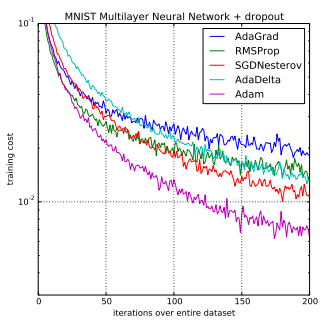
\includegraphics[width=0.5\textwidth]{capitulo_marcoteorico/adam}
    \caption{Rendimiento de algoritmos de optimización en la BD de MNIST}\label{fig:adam}
\end{figure}

\subsection{Arquitecturas}

En esta sección se describirán brevemente las arquitecturas seleccionadas para
la elaboración del modelo. Como veremos posteriormente, por las características
y elementos que contiene la \hyperlink{abbr}{BD} usada en este trabajo, se
realizarán tres experimentos basados en clasificación y segmentación. Siendo
VGG19 la elegida para el problema de clasificación binaria y multi-clase
mediante una búsqueda exhaustiva en todo el \emph{Zoológico de modelos} de
\textbf{Keras}; mientras que Unet es la que sugiere la literatura para el uso de
segmentación en imágenes citológicas. 

\subsubsection{VGG19}

Esta arquitectura fue inventada por el Grupo de Geometría Visual o VGG por sus
siglas en inglés de la Universidad de Oxford. VGG19 es una
\hyperlink{abbr}{ConvNet} entrenada en \emph{ImageNet} para clasificar más de
mil categorías distintas. Como resultado la red ha aprendido muchas
representaciones útiles y abstractas sobre muchas imágenes \cite{Simonyan2014}. 

VGG19 fue uno de los algoritmos con mejor rendimiento en el reto de
\emph{ImageNet} en el 2014 y mejoró por mucho el ganador del año anterior.
Siendo mejor que el ganador de la competencia de 2014, GoogLeNet en otras tareas
de \hyperlink{abbr}{VC}.

La innovación de VGG19 con respecto a sus competidores fue el uso de tres capas
con filtros $ 3 \times 3 $ en lugar una capa con filtros grandes como $11 \times
11$ usado en otras arquitecturas. Esto redujo la cantidad de parámetros
que la red tenía que aprender durante el entrenamiento. Suponiendo
1 filtro por capa y una capa en la entrada:
\leavevmode \\
\begin{itemize}
    \item 1 capa de filtro $11 \times 11$: $11 \times 11 = 121$ parámetros
    \item 5 capas de filtros $3 \times 3$: $3 \times 3 \times 5 = 45$ parámetros % 
    \smash{\raisebox{.5\dimexpr3\baselineskip+4\itemsep-1\parskip}{$\left.\rule{0pt}{.5\dimexpr4\baselineskip+3\itemsep+3\parskip}\right\}\text{63\% de reducción}$}}
  \end{itemize}
  \leavevmode \\
\begin{itemize}
\item 1 capa de filtro $7 \times 7$: $7 \times 7 = 49$ parámetros
\item 3 capas de filtros $3 \times 3$: $3 \times 3 \times 3 = 27$ parámetros % 
\smash{\raisebox{.5\dimexpr3\baselineskip+4\itemsep-1\parskip}{$\left.\rule{0pt}{.5\dimexpr4\baselineskip+3\itemsep+3\parskip}\right\}\text{45\% de reducción}$}}
\end{itemize}\leavevmode \\

\begin{itemize}
\item 1 capa de filtro $5 \times 5 $: $5 \times 5 = 25$ parámetros
\item 2 capas de filtros $3 \times 3$: $3 \times 3 \times 2 = 18$ parámetros % 
\smash{\raisebox{.5\dimexpr3\baselineskip+4\itemsep-1\parskip}{$\left.\rule{0pt}{.5\dimexpr4\baselineskip+3\itemsep+3\parskip}\right\}\text{28\% de reducción}$}}
\end{itemize}

Podemos ver en la \autoref{fig:vgg_diagram} como al ingresar una imagen
representada por un tensor de $256 \times 256 \times 3$, es procesada primero
por dos capas convolucionadas de tamaño $256 \times 256 \times 64$ para después
pasar por una capa \emph{MaxPool2D} y ser reducida a un tensor $128 \times 128
\times 64$. Las capas convolucionadas subsecuentes incrementarán la profundidad
del tensor en cada paso, mientras que las capas \emph{MaxPool2D} reducirán su
ancho y alto. Finalmente pasarán por dos capas densas de 1024 neuronas, cada una
con su capa de Dropout para terminar en una capa softmax de tantas neuronas como
clases se tienen.

\begin{figure}[H]
    \centering
    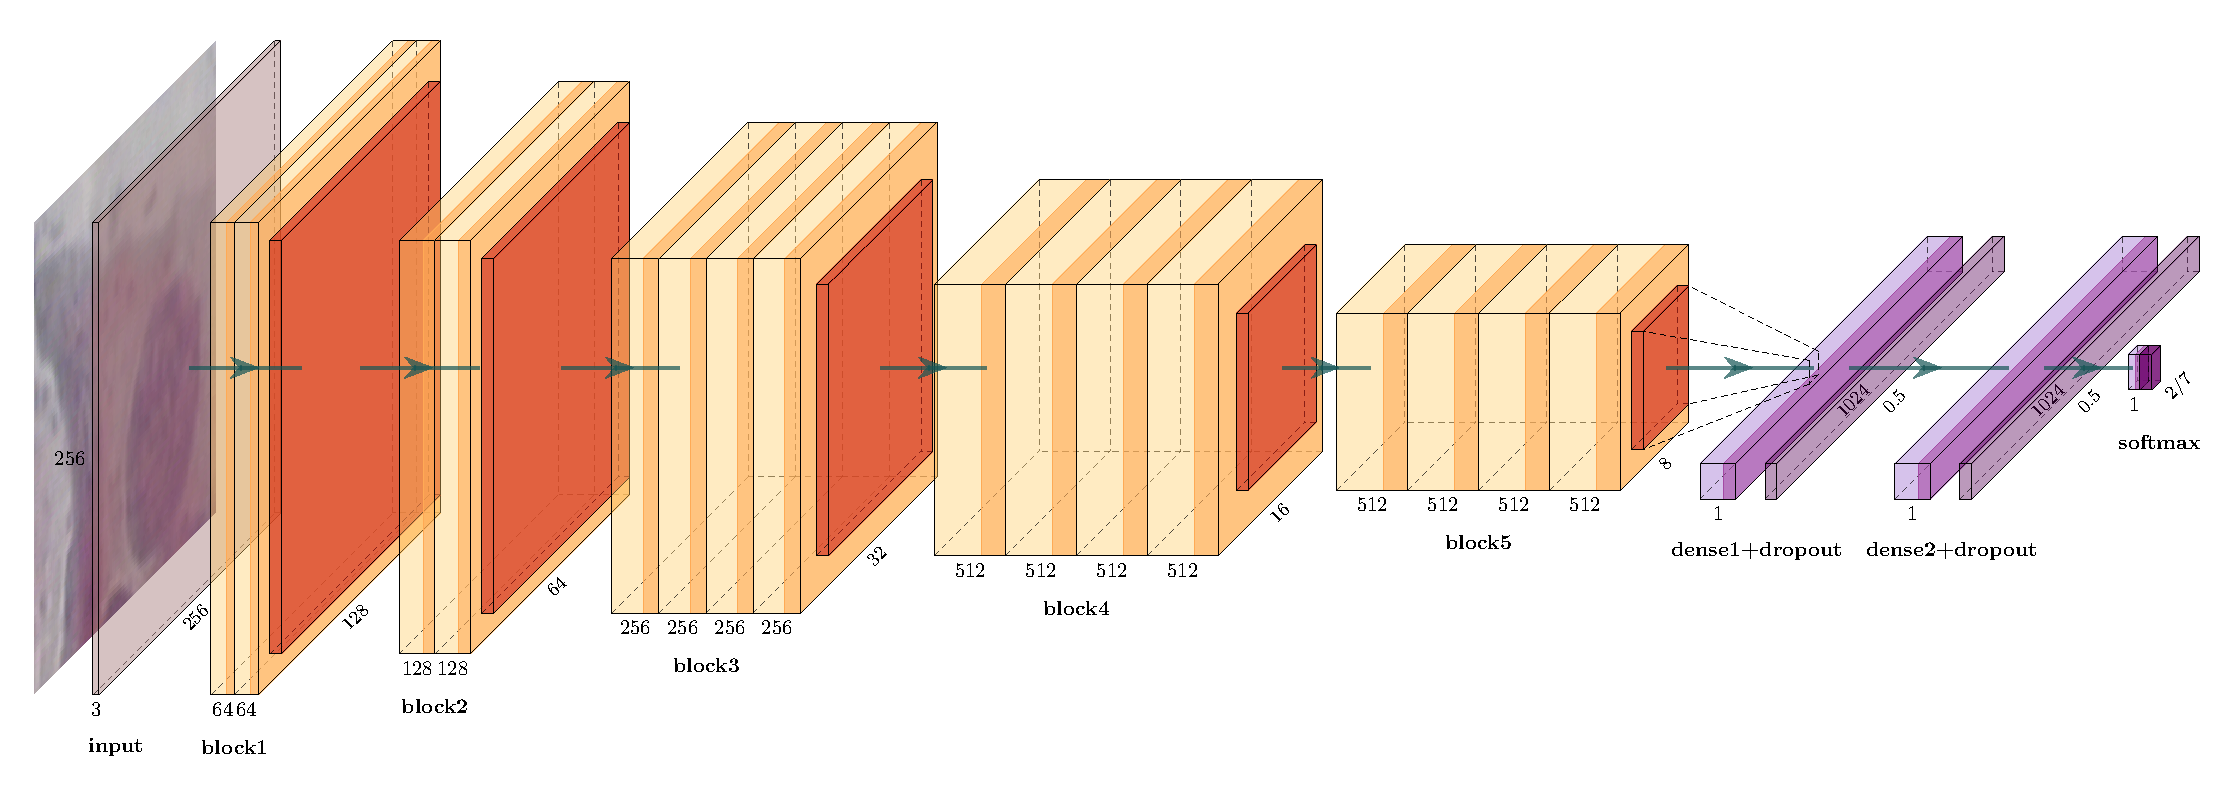
\includegraphics[width=\textwidth]{capitulo_marcoteorico/vgg19_test.pdf}
    \caption{Diagrama de la arquitectura VGG19}\label{fig:vgg_diagram}
  \end{figure}

La arquitectura final del modelo se presenta en la~\autoref{tabla:modelo}. Donde
se desglosan todas las capas de la arquitectura~\emph{VGG19}. Las capas
convolucionales están agrupadas en bloques junto con su \emph{MaxPool2D}. Se
muestra como los parámetros a aprender van aumentando conforme pasan los
bloques, culminando en aproximadamente 55 millones de parámetros, es decir,
números individuales pertenecientes a la matriz de pesos que se tienen que
ajustar.

\lstset{ 
  backgroundcolor=\color{white},   % choose the background color; you must add \usepackage{color} or \usepackage{xcolor}; should come as last argument
  basicstyle=\scriptsize,        % the size of the fonts that are used for the code
  breakatwhitespace=false,         % sets if automatic breaks should only happen at whitespace
  keepspaces=false,                 % keeps spaces in text, useful for keeping indentation of code (possibly needs columns=flexible)
  showspaces=false,                % show spaces everywhere adding particular underscores; it overrides 'showstringspaces'
  showstringspaces=false,          % underline spaces within strings only
  showtabs=false,                  % show tabs within strings adding particular underscores
  stepnumber=1,                    % the st
}
\begin{table}[H]
    \centering
    \begin{lstlisting}
        _________________________________________________________________
        Layer (type)                 Output Shape              Param #   
        =================================================================
        input_2 (InputLayer)         (None, 256, 256, 3)       0         
        _________________________________________________________________
        block1_conv1 (Conv2D)        (None, 256, 256, 64)      1792      
        _________________________________________________________________
        block1_conv2 (Conv2D)        (None, 256, 256, 64)      36928     
        _________________________________________________________________
        block1_pool (MaxPooling2D)   (None, 128, 128, 64)      0         
        _________________________________________________________________
        block2_conv1 (Conv2D)        (None, 128, 128, 128)     73856     
        _________________________________________________________________
        block2_conv2 (Conv2D)        (None, 128, 128, 128)     147584    
        _________________________________________________________________
        block2_pool (MaxPooling2D)   (None, 64, 64, 128)       0         
        _________________________________________________________________
        block3_conv1 (Conv2D)        (None, 64, 64, 256)       295168    
        _________________________________________________________________
        block3_conv2 (Conv2D)        (None, 64, 64, 256)       590080    
        _________________________________________________________________
        block3_conv3 (Conv2D)        (None, 64, 64, 256)       590080    
        _________________________________________________________________
        block3_conv4 (Conv2D)        (None, 64, 64, 256)       590080    
        _________________________________________________________________
        block3_pool (MaxPooling2D)   (None, 32, 32, 256)       0         
        _________________________________________________________________
        block4_conv1 (Conv2D)        (None, 32, 32, 512)       1180160   
        _________________________________________________________________
        block4_conv2 (Conv2D)        (None, 32, 32, 512)       2359808   
        _________________________________________________________________
        block4_conv3 (Conv2D)        (None, 32, 32, 512)       2359808   
        _________________________________________________________________
        block4_conv4 (Conv2D)        (None, 32, 32, 512)       2359808   
        _________________________________________________________________
        block4_pool (MaxPooling2D)   (None, 16, 16, 512)       0         
        _________________________________________________________________
        block5_conv1 (Conv2D)        (None, 16, 16, 512)       2359808   
        _________________________________________________________________
        block5_conv2 (Conv2D)        (None, 16, 16, 512)       2359808   
        _________________________________________________________________
        block5_conv3 (Conv2D)        (None, 16, 16, 512)       2359808   
        _________________________________________________________________
        block5_conv4 (Conv2D)        (None, 16, 16, 512)       2359808   
        _________________________________________________________________
        block5_pool (MaxPooling2D)   (None, 8, 8, 512)         0         
        _________________________________________________________________
        flatten_2 (Flatten)          (None, 32768)             0         
        _________________________________________________________________
        dense_4 (Dense)              (None, 1024)              33555456  
        _________________________________________________________________
        dropout_3 (Dropout)          (None, 1024)              0         
        _________________________________________________________________
        dense_5 (Dense)              (None, 1024)              1049600   
        _________________________________________________________________
        dropout_4 (Dropout)          (None, 1024)              0         
        _________________________________________________________________
        dense_6 (Dense)              (None, N)                 2050      
        =================================================================
        Total params: 54,631,490
        Trainable params: 34,607,106
        Non-trainable params: 20,024,384
        _________________________________________________________________
        
    \end{lstlisting}
    \caption{Parámetros de VGG19}
    \label{tabla:modelo}
\end{table}

\subsubsection{Unet}

U-net es una arquitectura diseñada para ser rápida y precisa. Ha tenido mejor
rendimiento en el reto ISBI que otras arquitecturas, esto en el área de
estructuras neuronales. Ha ganado el Grand Challenge for Computer-Automated
Detection fo Caries in Bitewing Radiography de ISBI en 2015 y cuenta con el
distinguido logro de haber ganado también el reto Cell Tracking Challenge del
mismo año en dos categorías distintas. Fue creada por los investigadores Olaf
Ronnenberger, Philipp Fishcer y Thomas Brox en el año de 2015.~\cite{Ronneberger2015}

En la~\autoref{fig:ejemplounet} se muestran aplicaciones de U-net para la
segmentación de imágenes citológicas dentro del reto ISBI. Las predicciones
fueron posteriormente post-procesadas para arrojar los contornos y las máscaras
que se observan en las imágenes.

\begin{figure}[H]
    \centering
    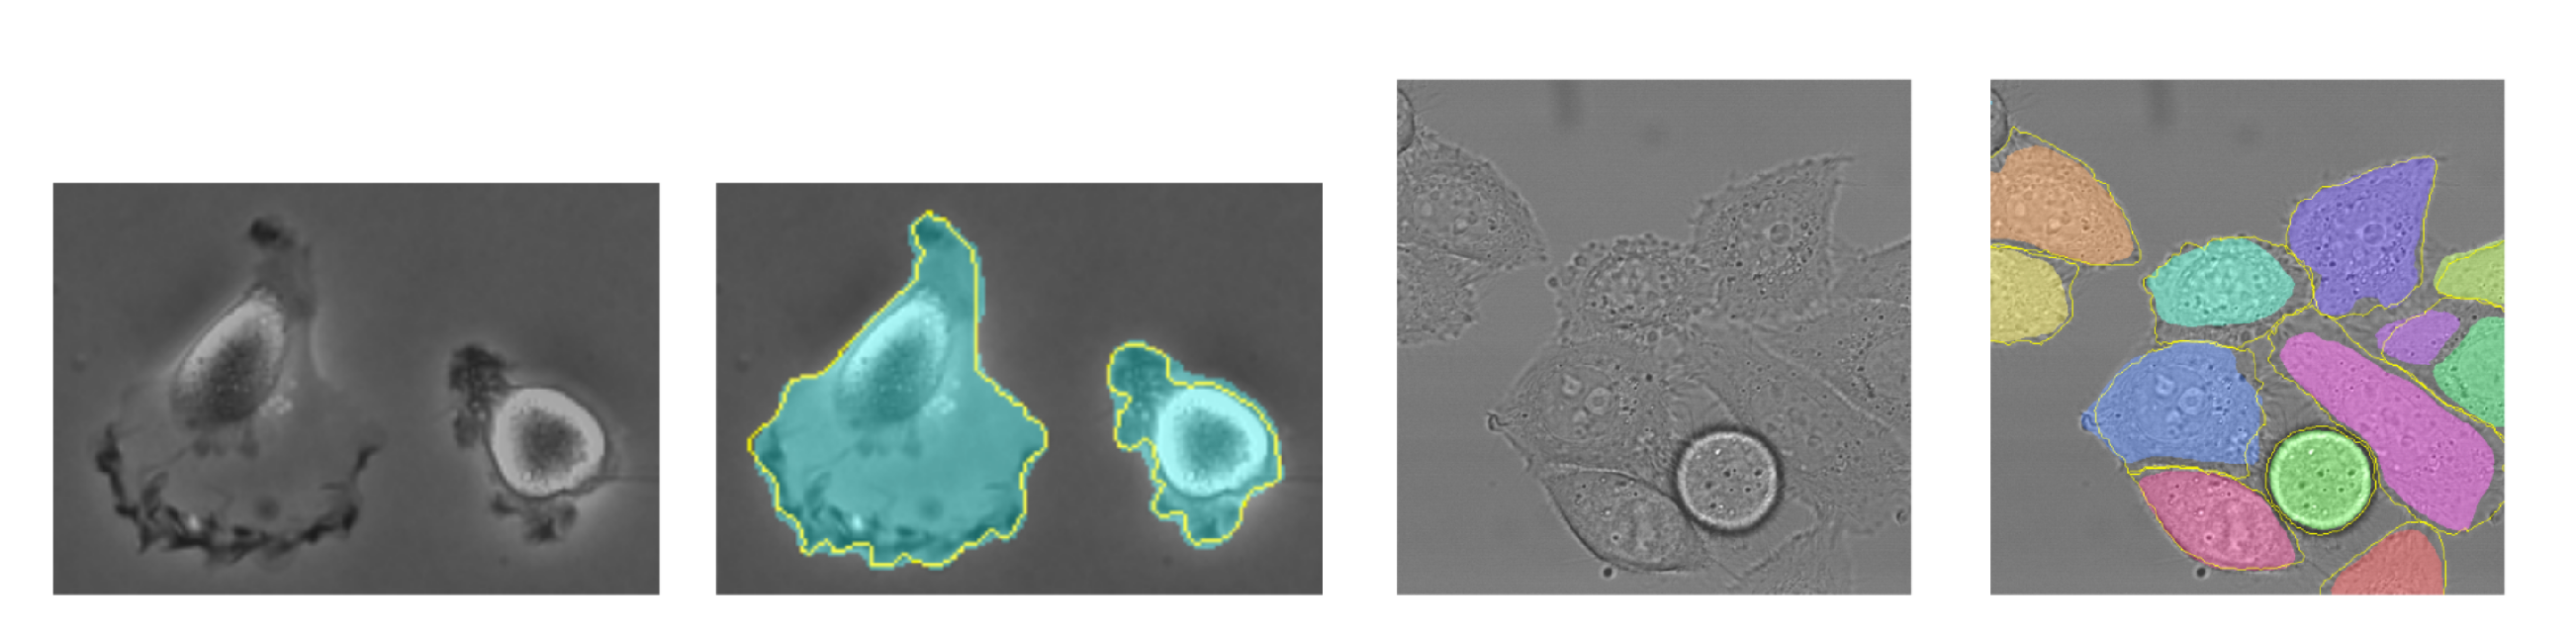
\includegraphics[scale=0.25]{capitulo_marcoteorico/ejemplo.pdf}
    \caption{Ejemplos de aplicaciones de U-net}\label{fig:ejemplounet}
\end{figure}

Las ventajas de U-net son las siguientes:

\begin{itemize}
    \item Combina la información de localización de la parte de contracción con la
    información contextual de la parte de expansión para obtener información
    general combinando ambas, lo cual es necesario para predecir un buen mapa
    de segmentación.
    \item No cuenta con una capa densa, esto permite que imágenes de distinto
    tamaño pueden ser usados como entrada.
    \item Se apoya muchísimo de la aumentación de datos.
    \item El modelo es relativamente pequeño (512 $\times$ 512 U-net - ca. 89mb).
    \item Cuenta son solo 2,164,593 parámetros totales.
\end{itemize}

La arquitectura de U-net (\autoref{fig:unet}) está construida sobre el concepto de 
Red Totalmente Convolucionada (FCN por sus siglas en inglés) y está modificada
de tal manera que tenga mejor rendimiento en la segmentación de imágenes médicas. 
Las diferencias entre ambas son relativamente sutiles, la primera arquitectura es
asimétrica e implementa ciertas funciones distintas en algunas de sus capas. U-net
es capaz de proveer información local a las capas posteriores para convertirlas
de nuevo a la escala de entrada.~\cite{DeepLearning}

\begin{figure}[H]
    \centering
    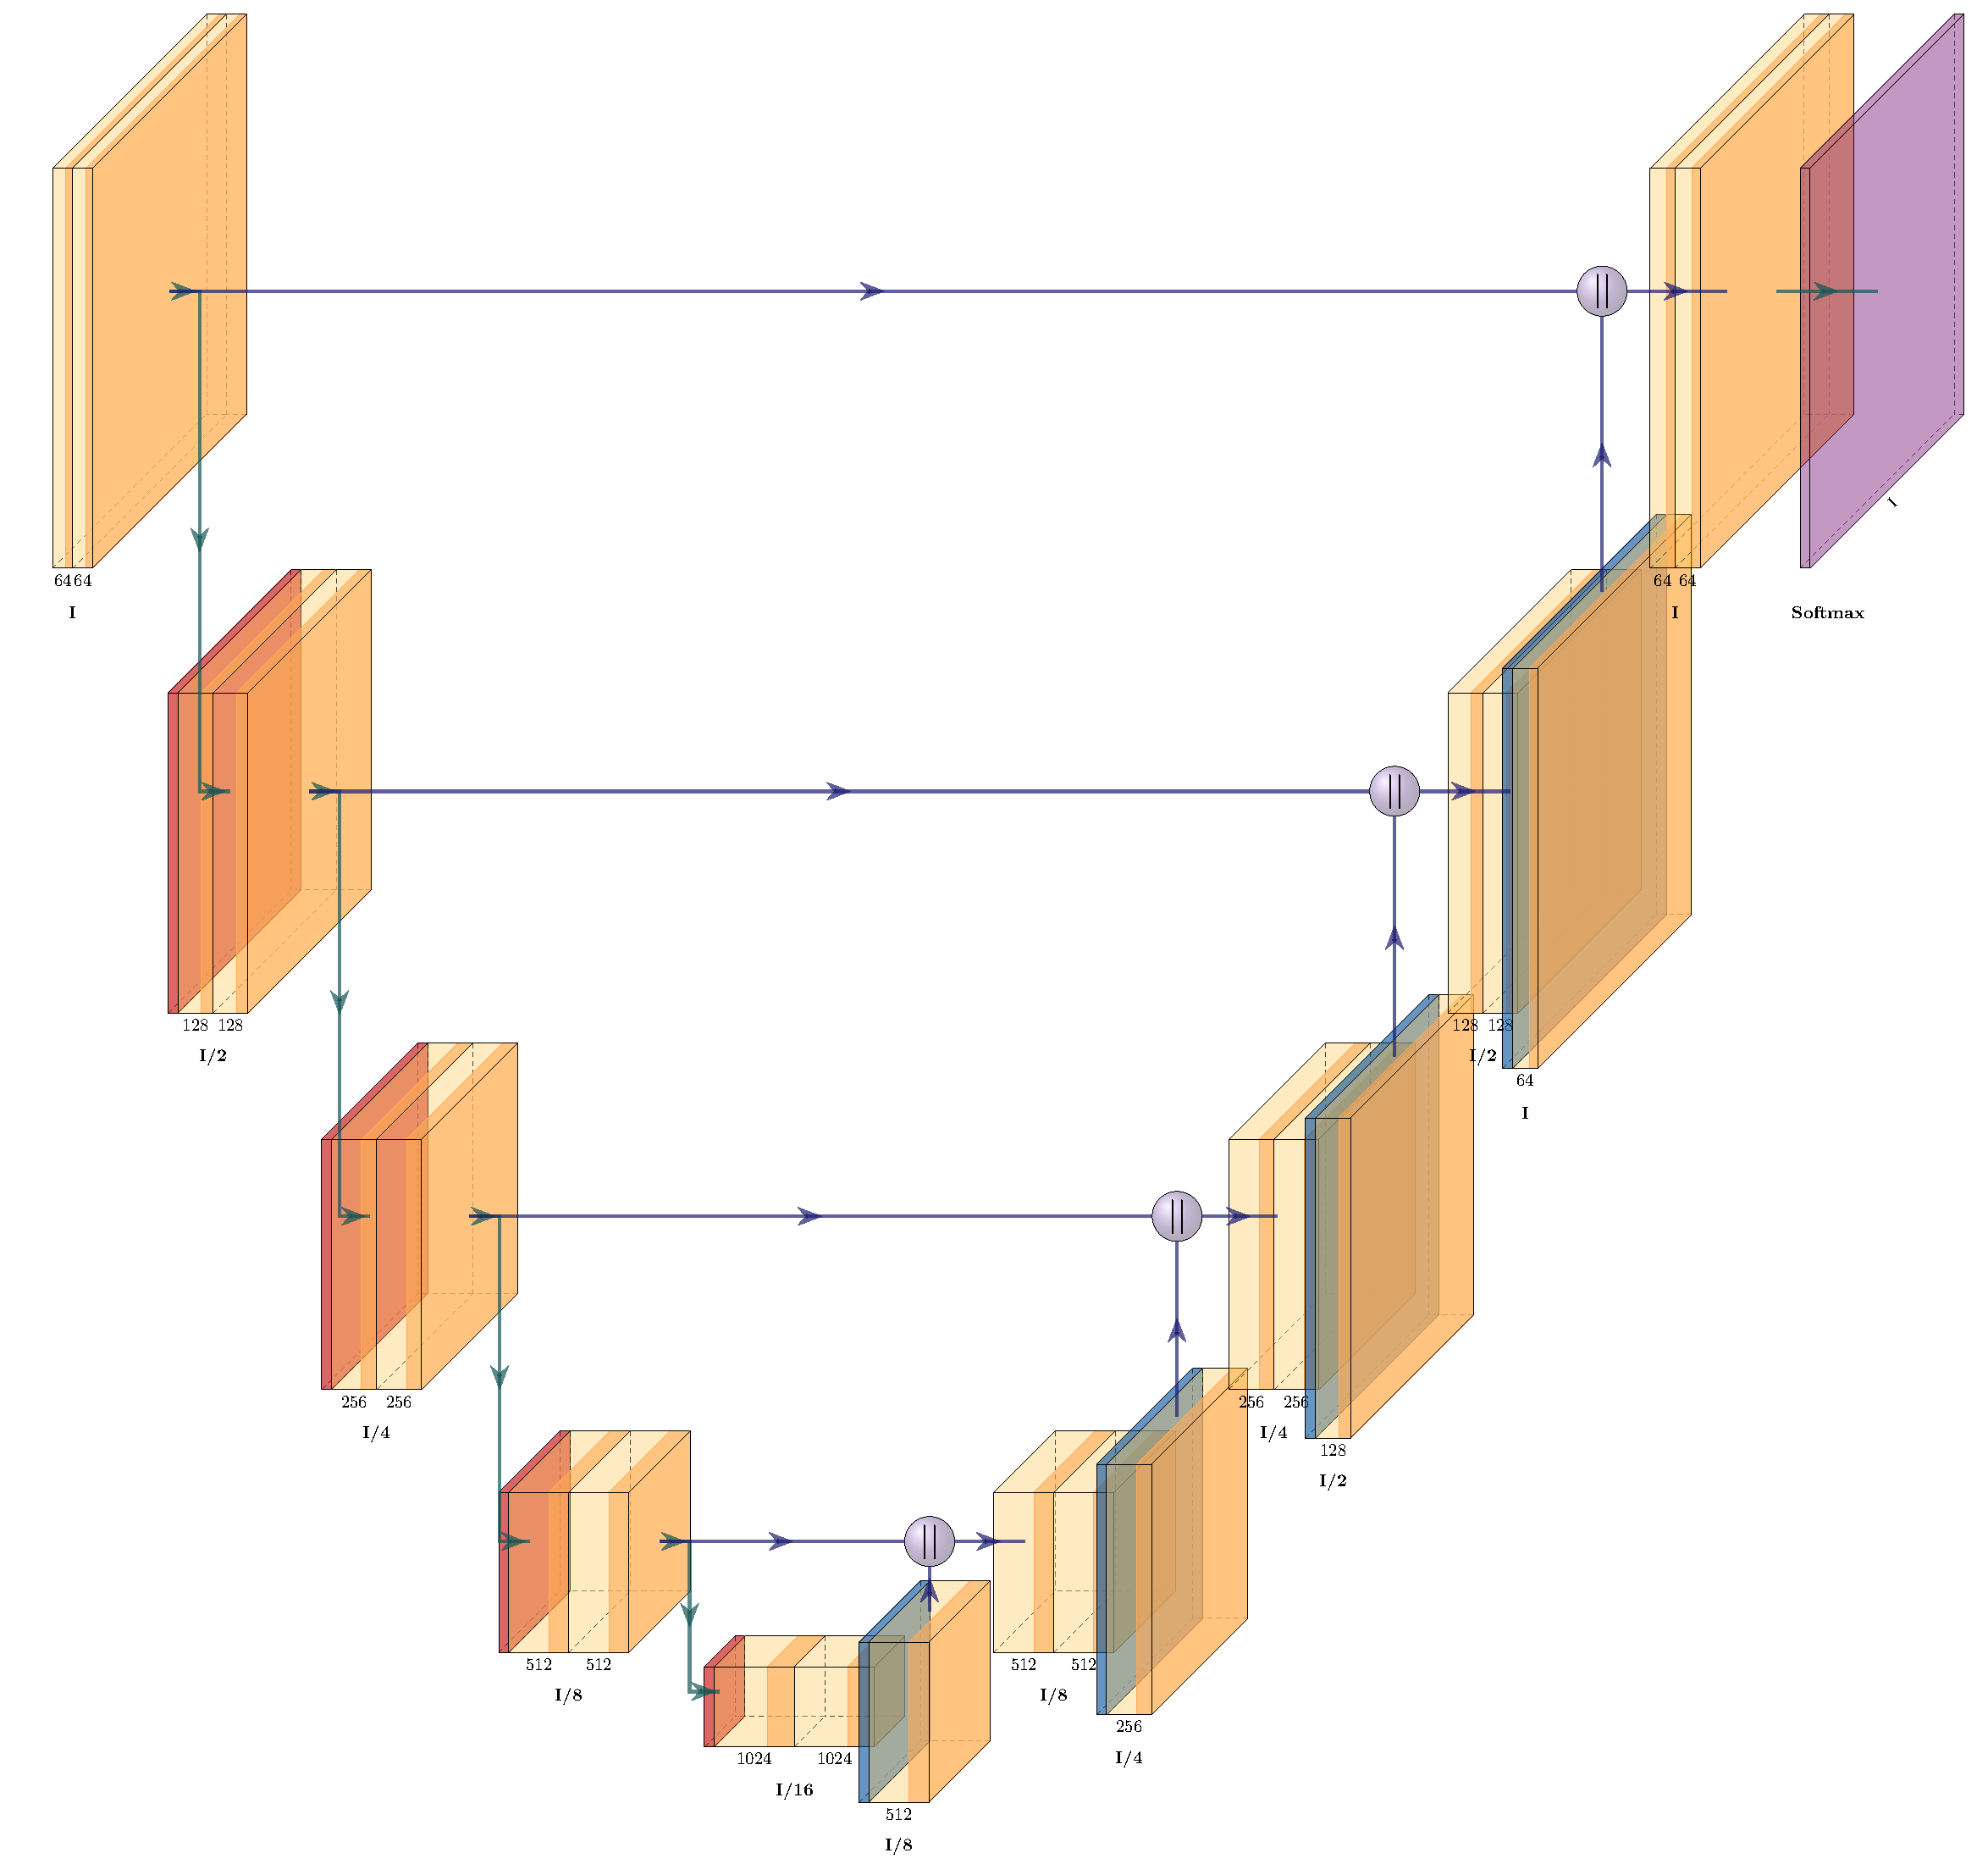
\includegraphics[scale=0.30]{capitulo_marcoteorico/Unet_ushape.pdf}
    \caption{La arquitectura U-net}\label{fig:unet}
\end{figure}

La arquitectura de U-net está dividida en tres partes:

\begin{enumerate}
    \item{Contracción:} Se compone por cuatro bloques y cada bloque está compuesto por:
        \begin{itemize}
            \item Capa convolucional 3 $\times$ 3 + función de activación (con normalización por lote).
            \item Capa convolucional 3 $\times$ 3 + función de activación (con normalización por lote).
            \item Capa de \emph{max pooling} 2 $\times$ 2.
        \end{itemize}
    \item{Cuello de botella:} Es el enlace entre las dos capas mostradas y su composición es bastante 
    sencilla: dos capas convolucionales con normalización por lote y dropout.
    \item{Expansión:} Al igual que la capa de contracción, se compone de cuatro partes:
    \begin{itemize}
        \item Cada deconvolucional con stride 2.
        \item Capa de concatenación que une las características con esta capa.
        \item  Capa convolucional 3 $\times$ 3 + función de activación (con normalización por lote).
        \item  Capa convolucional 3 $\times$ 3 + función de activación (con normalización por lote).
    \end{itemize}
\end{enumerate}

Se puede tonar que los pesos de las capas se están inicializando con la función
\emph{he normal}. La cual toma muestras de una distribución normal truncada
centrada en 0 y con una desviación estándar \(std =
\sqrt{\frac{2}{\mathbf{W_{n}}}}\), donde \(\mathbf{W_{n}}\) es el número de
unidades en el tensor de pesos.  Las funciones de activación se mantienen en
\emph{ReLU}.~\cite{He2015} 

A futuro podría ser posible reemplazar la fase de contracción por una arquitectura
convolucional como las vistas en el \emph{Zoológico de Modelos}, y configurar una función
que genere la fase de expansión dinámicamente en función a la arquitectura que se escoja 
para la contracción. El cuello de botella se mantendría inalterado.

Esto nos permitiría utilizar \hyperlink{abbr}{TL} para mejorar la precisión del
modelo. También se busca la forma de implementar completa segmentación
semántica, para células normales y anormales utilizando toda la imagen así como
revisar el problema de las siete clases distintas.

Al evaluar cualquier algoritmo de aprendizaje, especialmente en clasificación se
catalogan las predicciones en cuatro categorías: verdaderos positivos, falsos
positivos, verdaderos negativos y falsos negativos. Sin embargo, para casos de
predicción y segmentación de imágenes, a veces no se tiene el panorama lo
suficientemente claro para catalogar cada resultado en alguna de estas
categorías.

La Intersección sobre Unión (IOU), también conocida como el índice de Jaccard, es
un método para cuantificar el porcentaje de superposición entre la máscara
objetivo y la predicción. Esta métrica está relacionada con el coeficiente de Dice,
es por ello que lo usaremos como función de pérdida. 

Esta métrica mide el número de pixeles comunes entre la máscara y la predicción divididos
sobre el número total de pixeles en ambas imágenes, que generalmente tienen el 
mismo número de pixeles (\autoref{Intersection over Union}). 

\ecuacion{IoU = \frac{etiqueta \cap predicci\acute{o}n}{etiqueta \cup predicci\acute{o}n}}{Intersection over Union}

% \begin{equation}
%     \label{eq:iou}
%     IoU = \frac{etiqueta \cap predicci\acute{o}n}{etiqueta \cup predicci\acute{o}n}
% \end{equation}

La pérdida implementada en este modelo es implementa el coeficiente de Dice
(\autoref{Dice coefficient}), que es un estadístico que nos permite comparar que tan
similares son dos muestras. Se puede observar que es bastante similar al F1-Score
utilizado en el paradigma anterior.

\ecuacion{D = \frac{2*|etiqueta\cdot predicci\acute{o}n|}{ |etiqueta| + |predicci\acute{o}n| }}{Dice coefficient}

% \begin{equation}
%     \label{eq:dice}
%     D = \frac{2*|etiqueta\cdot predicci\acute{o}n|}{ |etiqueta| + |predicci\acute{o}n| } \\ 
% \end{equation}

La~\autoref{Dice Loss} muestra la fórmula completa de la pérdida. Notar
que implementa tanto el coeficiente de Dice como la entropía cruzada, en este caso
dos clases: núcleo y fondo.

\ecuacion{P\acute{e}rdida = \frac{1}{2} * entrop\acute{\imath}a - D}{Dice Loss}

% \begin{equation}
%     \label{eq:diceloss}
%     P\acute{e}rdida = \frac{1}{2} * entrop\acute{\imath}a - D
% \end{equation}


\subsubsection{Software}

Python es un lenguaje creado en 1990. Es un lenguaje del tipo interpretado, con
sistema de tipos dinámico, orientado a objetos, procedural, funcional,
imperativo, de código abierto e implementado en distintos tipos de compiladores
diseñados para situaciones altamente optimizadas.

Está diseñado para maximizar la legibilidad, omitiendo paréntesis, llaves y
corchetes excesivos, abogando por una estructura basada en la identación del
código. Lo cual otorga una legibilidad muy superior a alternativas más rápidas
como C++. 

El lenguaje es maduro y se encuentra en operación dentro de grandes
organizaciones, manejando todos los aspectos desde aplicaciones web hasta
análisis de datos e inteligencia artificial; temas en los que Python se ha
convertido en la opción en cuanto a análisis de datos, ciencia de datos,
aprendizaje automático. La ventaja de Python comparado con viejos competidores
como R o Matlab, es que es un lenguaje de propósito general, a diferencia de
lenguaje de dominio. Esto lo hace perfecto para ser integrado en prácticamente
todas las aplicaciones posibles desde web hasta control de vehículos autónomos. 

Frameworks como Django, permite a cualquier aplicación escrita en Python
interactuar con la web de manera tanto síncrona como asíncrona. Equiparando su
usabilidad con veteranos web como PHP. También, existe forma de implementar
Python en dispositivos móviles tanto de Apple como de Android; esto lo convierte
en un lenguaje completo y versátil.

Cuenta con módulos específicos para procesamiento numérico, tanto distribuido
como en paralelo. Nvidia, la empresa fabricante de los mejores
\hyperlink{abbr}{GPU}s, ha implementado una versión de su lenguaje de
programación \hyperlink{abbr}{CUDA} en Python, por lo cual entrenar redes
neuronales se puede hacer dentro de estos dispositivos. Incrementando en órdenes
de magnitud la velocidad de entrenamiento.

Existen muchos frameworks de software para trabajar con \hyperlink{abbr}{DL}.
Algunos son de paga como Matlab mientras que otros se basan en el paradigma del
software libre. \textbf{Tensorflow} es una biblioteca para el lenguaje
\emph{Python} para cómputo simbólico, programación diferenciable y flujo de
datos especialmente diseñada para implementar eficientemente algoritmos de
\hyperlink{abbr}{IA}. Fue desarrollada por Google para sus proyectos internos y
posteriormente ya madura fue lanzada al público. Es capaz de utilizar el poder
computacional de un \hyperlink{abbr}{GPU} y de optimizar un modelo ya entrenado
para su despliegue en un dispositivo móvil o \hyperlink{abbr}{SE}. Junto con
\textbf{Keras}, se conforma una plataforma completa de desarrollo de \hyperlink{abbr}{DL} que es a
la vez sumamente poderosa y sencilla. 


\begin{figure}[H]
    \centering
    
\includegraphics[width=0.5\textwidth]{capitulo_marcoteorico/tf}
    \caption{Tensorflow y Keras}\label{fig:tf}
\end{figure}